\documentclass[11pt,oneside]{article}
\usepackage[a4paper,margin=26mm,headheight=15pt]{geometry}
\usepackage[T1]{fontenc}
\usepackage[utf8]{inputenc}
\IfFileExists{libertinus.sty}{\usepackage{libertinus}}{\usepackage{lmodern}}
\usepackage{microtype}
\usepackage{amsmath,amssymb,amsthm,mathtools,mathrsfs,bm}
\usepackage{booktabs,longtable,array,tabularx,multirow}
\usepackage{graphicx}
\usepackage{caption}
\usepackage{xcolor}
\usepackage{enumitem}
\usepackage{fancyhdr}
\usepackage{titlesec}
\usepackage{listings}
\usepackage{xurl}
\usepackage[hypertexnames=false]{hyperref}
\usepackage[nameinlink,noabbrev]{cleveref}

\graphicspath{
  {assets/inverse_fabius_all_orders_package/results/}
  {assets/inverse_fabius_asymptotics_report/}
  {assets/inverse_fabius_asymptotics_package/figures/}
}

\definecolor{linkblue}{RGB}{25,75,135}
\definecolor{deepgreen}{RGB}{28,103,76}
\definecolor{shadegray}{RGB}{246,247,249}
\definecolor{rulegray}{RGB}{195,201,208}
\hypersetup{
  colorlinks=true,
  linkcolor=linkblue,
  citecolor=deepgreen,
  urlcolor=linkblue,
  pdftitle={All-Orders Endpoint Asymptotics for the Inverse Fabius Function},
  pdfsubject={Diagonal Lagrange-Buermann coefficients, saddle partition sums,
    phase-locked tomography, inverse derivatives, and the exact 2-adic
    completion of the Laplace exponent},
  pdfkeywords={Fabius function, inverse Fabius function, Lambert W, Lagrange
    inversion, Bell polynomials, Gamma-zeta fluctuation, Thue-Morse, 2-adic
    valuation, Mellin transform, resurgence}
}

\pagestyle{fancy}
\fancyhf{}
\fancyhead[L]{\small Inverse Fabius endpoint asymptotics}
\fancyhead[R]{\small\nouppercase{\leftmark}}
\fancyfoot[C]{\thepage}
\renewcommand{\headrulewidth}{0.4pt}
\titleformat{\section}{\Large\bfseries}{\thesection}{0.7em}{}
\titleformat{\subsection}{\large\bfseries}{\thesubsection}{0.7em}{}
\titleformat{\subsubsection}{\normalsize\bfseries}{\thesubsubsection}{0.7em}{}
\setcounter{secnumdepth}{3}
\setcounter{tocdepth}{2}
\setlist[itemize]{leftmargin=2em,itemsep=0.25em,topsep=0.4em}
\setlist[enumerate]{leftmargin=2.3em,itemsep=0.25em,topsep=0.4em}
\setlength{\emergencystretch}{3em}
\allowdisplaybreaks[2]
\numberwithin{equation}{section}

% ed.: alias counters so cleveref prints each environment's own name
% (with plain shared counters every \cref rendered as "theorem").
\usepackage{aliascnt}
\newcommand{\newsharedtheorem}[2]{%
  \newaliascnt{#1}{theorem}%
  \newtheorem{#1}[#1]{#2}%
  \aliascntresetthe{#1}%
}
\newtheorem{theorem}{Theorem}[section]
\newsharedtheorem{proposition}{Proposition}
\newsharedtheorem{lemma}{Lemma}
\newsharedtheorem{corollary}{Corollary}
\newsharedtheorem{identity}{Identity}
\newsharedtheorem{conjecture}{Conjecture}
\newsharedtheorem{problem}{Problem}
\theoremstyle{definition}
\newsharedtheorem{definition}{Definition}
\newsharedtheorem{algorithm}{Algorithm}
\newsharedtheorem{example}{Example}
\newsharedtheorem{obligation}{Formalization obligation}
\theoremstyle{remark}
\newsharedtheorem{remark}{Remark}
\newsharedtheorem{warning}{Warning}
\crefname{conjecture}{conjecture}{conjectures}
\Crefname{conjecture}{Conjecture}{Conjectures}
\crefname{problem}{problem}{problems}
\Crefname{problem}{Problem}{Problems}
\crefname{identity}{identity}{identities}
\Crefname{identity}{Identity}{Identities}
\crefname{algorithm}{algorithm}{algorithms}
\Crefname{algorithm}{Algorithm}{Algorithms}
\crefname{obligation}{formalization obligation}{formalization obligations}
\Crefname{obligation}{Formalization obligation}{Formalization obligations}
\crefname{warning}{warning}{warnings}
\Crefname{warning}{Warning}{Warnings}

\newcommand{\R}{\mathbb R}
\newcommand{\C}{\mathbb C}
\newcommand{\Q}{\mathbb Q}
\newcommand{\N}{\mathbb N}
\newcommand{\Z}{\mathbb Z}
\newcommand{\E}{\mathbb E}
\newcommand{\Prob}{\mathbb P}
\newcommand{\dd}{\,\mathrm d}
\newcommand{\e}{\mathrm e}
\newcommand{\ii}{\mathrm i}
\newcommand{\bigO}{\mathcal O}
\newcommand{\smallo}{o}
\newcommand{\eps}{\varepsilon}
\newcommand{\vtwo}{\nu_2}
\newcommand{\abs}[1]{\left\lvert #1\right\rvert}
\newcommand{\norm}[1]{\left\lVert #1\right\rVert}
\newcommand{\floor}[1]{\left\lfloor #1\right\rfloor}
\DeclareMathOperator{\Res}{Res}
\newcommand{\LambertW}{W}
\newcommand{\Up}{\operatorname{up}}
\newcommand{\Bell}{Y}
\newcommand{\Psihat}{\widehat\Psi}
\newcommand{\Csharp}{C_{\sharp}}
\newcommand{\CB}{C_{B}}
\newcommand{\Gzero}{G_0}
\newcommand{\repo}{\nolinkurl{Analysis/FabiusFunction/docs}}
\newcommand{\ind}{\mathbf 1}
\newcommand{\Hnum}{\mathsf H}

\newenvironment{statusbox}[1]{%
  \par\smallskip\noindent\begin{center}\begin{minipage}{0.94\textwidth}%
  \hrule\vspace{0.5em}\noindent\textbf{#1}\par\smallskip
}{%
  \vspace{0.5em}\hrule\end{minipage}\end{center}\smallskip
}

\lstdefinestyle{pythonstyle}{
  language=Python,
  basicstyle=\ttfamily\footnotesize,
  backgroundcolor=\color{shadegray},
  frame=single,
  rulecolor=\color{rulegray},
  columns=fullflexible,
  keepspaces=true,
  showstringspaces=false,
  breaklines=true,
  xleftmargin=0.7em,
  xrightmargin=0.7em,
  aboveskip=0.8em,
  belowskip=0.8em
}

\title{\bfseries All-Orders Endpoint Asymptotics\\
for the Inverse Fabius Function\\[0.45em]
\large Diagonal Lagrange--B\"urmann coefficients, saddle partition sums,\\
phase-locked tomography, inverse derivatives,\\
and the exact $2$-adic completion of the Laplace exponent}
\author{Consolidated frontier volume for Vladimir Reshetnikov's \texttt{ProveIt} project}
\date{28 August 2026}

\begin{document}
\maketitle

\begin{abstract}
\noindent
Let $F$ be the Fabius distribution function and $G=F^{-1}$ its
quantile.  The corpus proves an all-orders small-$x$ expansion of
$\log F$ in the exact lower-Lambert phase, with a one-periodic
Gamma--zeta fluctuation $\Psi$ and periodic saddle coefficients
$A_j$, and its inverse volume derives the first two endpoint
corrections of $G$ together with a triangular all-orders recursion.
This volume consolidates two independently written reports that close
the remaining coefficient-level gaps --- by, in several places,
proving the same theorems, which are stated here once with the merged
proofs and cross-validated constants.

With $T=\log(1/y)$, $L=\log2$, $\rho=\sqrt{2T/L}$, $\ell=\log\rho$,
$\beta=1/L+\tfrac12$, and the fast phase $\theta=\rho+\beta$, the
quantile satisfies, for every fixed $N$,
\[
 G(y)=\Gzero(y)\Bigl(1+\sum_{n=1}^{N}
 \frac{g_n(\ell,\theta)}{\rho^{\,n}}
 +\bigO_N\bigl((1+\ell)^{N+1}\rho^{-N-1}\bigr)\Bigr),
 \qquad
 \Gzero(y)=\frac{\sqrt T}{\e\sqrt L}\,\e^{-\sqrt{2LT}},
\]
with coefficients polynomial in $\ell$ and real-analytic one-periodic
in $\theta$.  A catalytic-variable Lagrange--B\"urmann inversion
gives every phase, logarithmic, and multiplicative coefficient by one
finite nonrecursive extraction; a direct partial-Bell formula gives
$g_n$ straight from the phase coefficients.  Structure laws follow:
the universal highest logarithm $[\ell^{\,n}]g_n=1/(2^{n}n!)$; the
newest-jet transfer
$[\Psi^{(2n-2)}]g_n=(-1)^{n}/(2^{n-1}(n-1)!\,L^{2n-2})$; explicit
Gamma--zeta convolutions for every Fourier mode with a common
analyticity strip $\abs{\Im\theta}<\pi/(2L)$; phase-locked quantile
sequences and coefficient tomography; an all-orders elasticity
recurrence; and, for each fixed $m$, the two-term derivative law with
harmonic-number correction.  The explicit third correction lowers the
relative error on exact dyadic quantiles $y_n=F(2^{-n})$ to
$4.9\times10^{-8}$ at $n=160$.

On the forward side, the complete Gaussian saddle correction is a
finite constrained partition sum (including the Bromwich
$1/t$ factor) that specializes to the Mills-ratio coefficients ---
completing an explicit pipeline
$\Psi\to\{\varkappa_r\}\to\{C_n\}\to\{\Lambda_n\}\to\{A_j\}\to
\{d_n\}\to\{g_n\}$.  And the Laplace exponent
$K=\log\E\,\e^{-tX}$ admits the \emph{exact} decomposition
\[
 K(t)=-\frac{\log^2t}{2L}+\frac12\log t-\CB
 +\Psi(\log_2t)+B(t),
 \qquad
 B(t)=\sum_{n\ge1}\frac{2^{\vtwo(n)+1}-1}{n}\,\e^{-nt},
\]
whose $2$-adically weighted Bose tail has Mahler equation, Dirichlet
series $\zeta(s+1)/(1-2^{-s})$, and a Mellin bridge showing that the
periodic phase and the exponentially small dyadic sectors are the two
faces of one kernel --- the concrete seed of an exponentially
improved inverse theory.

Finally, a Wright-omega \emph{resummation} of the carrier absorbs the
entire nonperiodic quadratic--linear--constant--logarithmic phase:
with $w$ defined through
$\omega\bigl(4(T+\Csharp+L\beta^{2}/2)+\log 2L\bigr)$, the expansion
$G/G_W\sim1+\sum g_m(w+\beta)w^{-m}$ has \emph{bounded periodic
coefficients with no logarithms at any order}, a clean
$w^{-N-1}$ remainder, the strikingly simple low orders
$g_1=-\Psi$ and $h_2=\tfrac5{24}+\cdots$, a convergent bare-skeleton
reversion (inversion is not the source of divergence), a conditional
Gevrey-one transfer theorem, and third-order accuracy
$1.1\times10^{-9}$ at $n=160$ on the exact dyadic quantiles ---
$43$ times better than the third $\rho$-order.  Provenance of the
absorbed sources, with SHA-256 hashes and the cross-validation
record, is in \cref{sec:provenance-inv}.
\end{abstract}

\clearpage
\tableofcontents
\clearpage

\section*{Provenance and merge conventions}
\addcontentsline{toc}{section}{Provenance and merge conventions}

This volume is an editorial consolidation (28 August 2026) of three
drafts of the fourth, fifth, and sixth waves that attack the same
problem and overlap heavily: the first two both prove the closed
Lagrange--B\"urmann coefficient formula, the universal highest
logarithm, the explicit third correction, and the all-orders
elasticity recurrence, and the third re-derives the same diagonal
calculus in a resummed normalization.  Each shared theorem is stated
once; where the sources' formulas could be compared they were
verified to agree exactly (notably the third correction $d_3$,
derived independently in different groupings; the elasticity
recurrence; and the carrier-invariant highest-derivative constants);
and each source's unique material --- the structure laws, Fourier
algebra, tomography, and derivative hierarchy of one; the saddle
partition engine and $2$-adic completion of another; the
Wright-omega log-free carrier of the third --- keeps its own
chapter.
\Cref{sec:provenance-inv} records the sources with SHA-256 hashes and
the deduplication detail; supporting files are under
\nolinkurl{assets/}.

\begin{statusbox}{Status discipline}
Theorems have complete proofs here or explicit citations; the
repository inputs (the forward all-orders expansion, $\Psi$,
$\Csharp$, $A_1$, the forward top-jet law, and the first two inverse
corrections with the triangular engine of the
\emph{Inverse and Sampling Frontiers} volume) are imported, not
reproved.  ``New'' means absent from the audited corpus snapshots
under the normalizations used there; no unqualified worldwide
priority is claimed.  Conjectures and problems are labeled; nothing
here is formalized in Lean yet.
\end{statusbox}

\subsection*{Notation}

\begin{center}
\small
\begin{tabular}{@{}llll@{}}
\toprule
$F$, $G=F^{-1}$ & Fabius function and quantile &
$L$ & $\log2$\\
$\beta$ & $1/L+\tfrac12$ &
$T$ & $\log(1/y)$\\
$\rho$ & $\sqrt{2T/L}$; \ $z=1/\rho$ &
$\ell$ & $\log\rho$\\
$\theta$ & $\rho+\beta$ (mod $1$ in periodic functions) &
$\lambda(x)$ & $-\LambertW_{-1}(-Lx)/L$, so $x=\lambda\e^{-L\lambda}$\\
$\Psi$ & mean-zero periodic Gamma--zeta fluctuation &
$A_j$ & periodic forward saddle coefficients\\
$D$ & $\lambda(G(y))-\rho-\beta=\sum d_nz^{n}$ &
$h_n$, $g_n$ & coefficients of $\log(G/\Gzero)$, $G/\Gzero$\\
$K(t)$ & $\log\E\,\e^{-tX}$ (Laplace exponent) &
$B(t)$ & dyadic Bose tail \eqref{eq:B-2adic}\\
$\varkappa_r$ & $s^{r}K^{(r)}(s)$ at the saddle &
$\varrho_r$ & $\varkappa_r/\varkappa_2$\\
$\Bell_n$, $\Bell_{n,k}$ & complete/partial exponential Bell &
$\Hnum_r$ & harmonic number $\sum_{j\le r}1/j$\\
\bottomrule
\end{tabular}
\end{center}
The constants
$\Csharp=\frac{6\gamma^{2}+12\gamma_1-\pi^{2}}{12L}
-\frac{7L}{12}-\frac12\log\pi$ and
$\CB=\frac{L}{12}+\frac{\pi^{2}-6\gamma^{2}-12\gamma_1}{12L}$
(Euler $\gamma$, first Stieltjes $\gamma_1$) satisfy the compact
relation $\Csharp+\CB=-\tfrac12\log(2\pi)$, proved with the
$2$-adic completion in \cref{sec:dyadic-completion}.

\section{Imported inputs and the two-scale inverse problem}
\label{sec:inputs}

\subsection{Forward input}

With $X=\sum_{j\ge1}2^{-j}U_j$ ($U_j$ i.i.d.\ uniform on $[0,1]$) and
$F(x)=\Prob(X\le x)$, the Laplace transform and exponent are
\begin{equation}
 M(t)=\E\,\e^{-tX}
 =\prod_{j\ge1}\frac{1-\e^{-t/2^{j}}}{t/2^{j}},
 \qquad
 K(t)=\log M(t),
 \label{eq:K-def}
\end{equation}
and the Bromwich integral
$F(x)=\frac1{2\pi\ii}\int_{(\sigma)}t^{-1}\exp(xt+K(t))\dd t$ is the
analytic source of the saddle expansion.  For small $x>0$ the exact
lower-Lambert phase is
$\lambda(x)=-\LambertW_{-1}(-Lx)/L$, i.e.\
$x=\lambda\e^{-L\lambda}$ exactly, and the repository's forward
theorem states: for every fixed $N\ge1$,
\begin{equation}
 \log F(x)=
 -\frac L2\lambda^{2}+L\beta\lambda-\frac12\log\lambda
 +\Csharp+\Psi(\lambda)
 +\sum_{j=1}^{N-1}\frac{A_j(\lambda)}{\lambda^{j}}
 +\bigO_N\bigl(\lambda^{-N}\bigr),
 \label{eq:forward-all-orders}
\end{equation}
uniformly in the phase, with every $A_j$ a bounded smooth one-periodic
differential polynomial in the Gamma--zeta fluctuation
\begin{equation}
 \Psi(u)=\sum_{k\ne0}\Psihat(k)\,\e^{2\pi\ii ku},
 \qquad
 \Psihat(k)=-\frac{\Gamma(-\chi_k)\,\zeta(1-\chi_k)}{L},
 \qquad
 \chi_k=\frac{2\pi\ii k}{L},
 \label{eq:Psi-Fourier}
\end{equation}
$\Psihat(0)=0$.  The explicit first correction and the forward
top-jet law are
\begin{equation}
 A_1(u)=\frac1{24}+\frac1{2L}
 -\frac{\Psi''(u)+\Psi'(u)^{2}}{2L^{2}},
 \qquad
 [\Psi^{(2j)}]A_j=\frac{(-1)^{j}}{2^{j}j!\,L^{2j}}.
 \label{eq:A1-and-topjet}
\end{equation}
The second correction, needed for the third inverse order, is
\begin{equation}
 A_2=\frac{P_1}{24L}+\frac{2P_1+1}{4L^{2}}
 -\frac{P_1^{3}+3P_1^{2}+3P_1P_2+3P_2+P_3}{6L^{3}}
 +\frac{4P_1^{2}P_2+4P_1P_3+2P_2^{2}+P_4}{8L^{4}},
 \label{eq:A2}
\end{equation}
with $P_r=\Psi^{(r)}(\theta)$, and
$A_1'=-(P_3+2P_1P_2)/(2L^{2})$.

\subsection{Inverse prior art}

The corpus's inverse volume establishes, and this volume imports: the
leading factor and first two phase corrections
\begin{equation}
 d_1=\frac{\beta^{2}}2
 +\frac{\Csharp+\Psi(\theta)-\tfrac12\ell}{L},
 \qquad
 d_2=\frac{\Psi'(\theta)\,d_1+A_1(\theta)-\tfrac12\beta}{L};
 \label{eq:d1-d2}
\end{equation}
the logarithmic corrections
$h_1=\tfrac12\ell+\kappa_0-\Psi(\theta)$ with
$\kappa_0=\beta-\tfrac L2\beta^{2}-\Csharp$, and $h_2$; the
nondegenerate first normalized cluster interval; the two-term
elasticity; and a triangular all-orders recursion.  The consolidated
results below convert that recursion into closed formulas and extend
every structural layer.

\subsection{The two-scale problem}

For $y\downarrow0$ set
$T,\rho,z,\ell,\theta$ as in the notation table and
\begin{equation}
 \Gzero(y)=\rho\,\e^{-L\rho-L\beta}
 =\frac{\sqrt T}{\e\sqrt L}\,\e^{-\sqrt{2LT}},
 \qquad
 \lambda(G(y))=\rho+\beta+D,
 \qquad
 D=\sum_{n\ge1}d_nz^{n}.
 \label{eq:G0-D}
\end{equation}
Substituting $\lambda=\rho+\beta+D$ into
\eqref{eq:forward-all-orders} and using
$-\tfrac L2\lambda^{2}+L\beta\lambda
=-T-L\rho D+\tfrac L2\beta^{2}-\tfrac L2D^{2}$ (the quadratic
collapses exactly because $T=L\rho^{2}/2$) reduces
$\log F(G(y))=-T$ to the fixed-point equation
\begin{equation}
 \boxed{\;D=z\,\Phi(z,D),\;}
 \qquad
 \Phi(z,w)=-\frac1L\mathcal R(z,w),
 \label{eq:fixed-point}
\end{equation}
with the formal residual
\begin{equation}
 \mathcal R(z,w)=
 -\frac L2\beta^{2}+\frac L2w^{2}+\frac12\ell
 +\frac12\log(1+\beta z+zw)
 -\Csharp-\Psi(\theta+w)
 -\sum_{j\ge1}\frac{A_j(\theta+w)\,z^{j}}{(1+\beta z+zw)^{j}}.
 \label{eq:R-def}
\end{equation}
Coefficients are computed in the two-scale ring
$\mathscr A[\ell][[z]]$, where $\mathscr A$ is the differential
algebra of one-periodic functions generated by $\Psi$ and the $A_j$:
$\ell$ and $\theta$ are treated as independent coefficient variables
and only afterwards evaluated at $\log\rho$ and $\rho+\beta$.  This
convention is forced, not cosmetic: $\theta$ winds around the circle
and $\ell$ is unbounded, so expanding either as a slow series would
destroy terms at their own order --- there is no phase-free complete
expansion (\cref{sec:structure}), and the correct coefficient space
is $\R[\ell]\otimes C^\infty(\R/\Z)$.

\begin{theorem}[All-orders inverse endpoint expansion]
\label{thm:all-orders}
For every fixed $N\ge1$ there are unique coefficients
$d_n,h_n,g_n\in\mathscr A[\ell]$ ($1\le n\le N$), polynomials in
$\ell$ with real-analytic one-periodic coefficients, such that as
$y\downarrow0$, uniformly in the phase,
\begin{align}
 \lambda(G(y))
 &=\rho+\beta+\sum_{n=1}^{N}\frac{d_n(\ell,\theta)}{\rho^{n}}
 +\bigO_N\Bigl(\frac{(1+\ell)^{N}}{\rho^{N+1}}\Bigr),
 \label{eq:phase-expansion}\\
 \log\frac{G(y)}{\Gzero(y)}
 &=\sum_{n=1}^{N}\frac{h_n(\ell,\theta)}{\rho^{n}}
 +\bigO_N\Bigl(\frac{(1+\ell)^{N}}{\rho^{N+1}}\Bigr),
 \qquad
 \frac{G(y)}{\Gzero(y)}
 =1+\sum_{n=1}^{N}\frac{g_n(\ell,\theta)}{\rho^{n}}
 +\bigO_N\Bigl(\frac{(1+\ell)^{N+1}}{\rho^{N+1}}\Bigr).
 \label{eq:G-expansion}
\end{align}
$d_n$ depends only on $\Psi,A_1,\dots,A_{n-1}$ and finitely many of
their derivatives.  By reflection, $G(1-y)=1-G(y)$ transfers every
formula to the right endpoint.
\end{theorem}

\begin{proof}
Substituting the truncation $D^{[N]}=\sum_{n\le N}d_nz^{n}$ into
\eqref{eq:fixed-point} and cancelling $z,\dots,z^{N}$ determines the
$d_n$ uniquely and triangularly ($D$ enters multiplied by $z$);
polynomial dependence on $\ell$ follows because the only explicit
$\ell$ in $\Phi$ is affine, and periodic analyticity from closure of
$\mathscr A$ (\cref{sec:fourier}).  The residual at $D^{[N]}$ is
$\bigO_N((1+\ell)^{N}z^{N})$, while on the connecting segment
$\partial_w\bigl(\tfrac Lzw+\mathcal R\bigr)=\tfrac Lz+\bigO_N(1)$;
the mean-value theorem gains one power of $z$ and proves
\eqref{eq:phase-expansion} (details in
\cref{app:proof-details}).  The exact Lambert identity gives
\begin{equation}
 \frac{G}{\Gzero}=(1+\beta z+zD)\,\e^{-LD},
 \qquad
 H:=\log\frac{G}{\Gzero}=\log(1+\beta z+zD)-LD,
 \label{eq:ratio-exact}
\end{equation}
and formal composition and exponentiation give
\eqref{eq:G-expansion}, the extra $(1+\ell)$ bounding the first
omitted complete Bell polynomial.
\end{proof}

\section{The diagonal Lagrange--B\"urmann calculus}
\label{sec:diagonal}

The triangular recursion computes order $n$ only after all lower
orders.  A catalytic variable turns the same fixed point into a
closed finite extraction at any single prescribed order --- the
central shared theorem of the two absorbed sources.

\begin{theorem}[Diagonal coefficient formulas]
\label{thm:diagonal}
For every $n\ge1$,
\begin{equation}
 \boxed{\;
 d_n=\sum_{k=1}^{n}\frac1k\,
 [z^{\,n-k}w^{\,k-1}]\;\Phi(z,w)^{k}
 =\sum_{k=1}^{n}\frac{(-1)^{k}}{k\,L^{k}}\,
 [z^{\,n-k}w^{\,k-1}]\;\mathcal R(z,w)^{k},
 \;}
 \label{eq:diagonal-dn}
\end{equation}
a finite formula: only the $z^{\,n-1}$-truncation of $\Phi$, the jets
$\Psi,\dots,\Psi^{(n-1)}$, and $A_1,\dots,A_{n-1}$ enter.  More
generally, for any formal $K(z,w)$,
\begin{equation}
 [z^{n}]\,K(z,D(z))
 =[z^{n}]\,K(z,0)
 +\sum_{k=1}^{n}\frac1k\,
 [z^{\,n-k}w^{\,k-1}]\;
 \partial_wK(z,w)\,\Phi(z,w)^{k},
 \label{eq:diagonal-composition}
\end{equation}
which with $K=\log(1+\beta z+zw)-Lw$ and
$K=(1+\beta z+zw)\e^{-Lw}$ gives closed diagonal formulas for
$h_n$ and $g_n$ directly.
\end{theorem}

\begin{proof}
Let $W(t,z)$ solve $W=t\,\Phi(z,W)$.  For fixed $z$, ordinary
Lagrange--B\"urmann inversion in $t$ gives
$[t^{k}]W=\tfrac1k[w^{k-1}]\Phi(z,w)^{k}$ and the composition form
$K(z,W)=K(z,0)+\sum_k\tfrac{t^{k}}k[w^{k-1}]\partial_wK\cdot\Phi^{k}$.
Since $D(z)=W(z,z)$, set $t=z$ and extract total degree $n$.
Finiteness: a term with Lagrange index $k$ asks for
$z^{\,n-k}w^{\,k-1}$, so no $A_jz^{j}$ with $j>n-k$ and at most $k-1$
phase derivatives occur.
\end{proof}

Expanding $\Phi=\sum\phi_{r,s}z^{r}w^{s}$ gives the fully unrolled
partition form
\[
 d_n=\sum_k\tfrac1k
 \sum_{r_1+\dots+r_k=n-k,\;s_1+\dots+s_k=k-1}
 \prod_j\phi_{r_j,s_j}
\]
--- convenient for proofs, while
\eqref{eq:diagonal-dn} is convenient for implementation.

\begin{theorem}[Direct partial-Bell formula for $g_n$]
\label{thm:direct-gn}
With $x_j=j!\,d_j$ and the partial Bell normalization
$(\sum_jd_jz^{j})^{k}
=\sum_{n\ge k}\frac{k!}{n!}\Bell_{n,k}(x_1,x_2,\dots)z^{n}$,
\begin{equation}
 \boxed{\;
 g_n=\frac1{n!}\sum_{k=1}^{n}(-L)^{k}\Bell_{n,k}
 +\frac{\beta}{(n-1)!}\sum_{k=0}^{n-1}(-L)^{k}\Bell_{n-1,k}
 +\frac1{(n-1)!}\sum_{k=1}^{n-1}k\,(-L)^{k-1}\Bell_{n-1,k},
 \;}
 \label{eq:gn-direct}
\end{equation}
all $\Bell_{m,k}=\Bell_{m,k}(x_1,x_2,\dots)$; combined with
\eqref{eq:diagonal-dn} this is a nonrecursive finite formula for the
arbitrary-order multiplicative coefficient.  The
logarithmic-to-multiplicative conversion is the complete-Bell
identity $g_n=\frac1{n!}\Bell_n(1!h_1,\dots,n!h_n)$, i.e.\
$ng_n=\sum_{j\le n}jh_jg_{n-j}$.
\end{theorem}

\begin{proof}
Expand the exact factorization \eqref{eq:ratio-exact}: the three
lines are $[z^{n}]\e^{-LD}$, $[z^{n-1}]\beta\e^{-LD}$, and
$[z^{n-1}]D\e^{-LD}$, each a standard partial-Bell expansion.
\end{proof}

\begin{algorithm}[Arbitrary-order symbolic generation]
\label{alg:generation}
Fix an output order $N$: obtain $A_1,\dots,A_{N-1}$ (from
\eqref{eq:A1-and-topjet}--\eqref{eq:A2} or the saddle pipeline of
\cref{sec:saddle}); Taylor-expand $\Psi(\theta+w)$, $A_j(\theta+w)$
only as far as the bidegrees require; truncate $\Phi$ at
$z^{N-1}$; evaluate \eqref{eq:diagonal-dn} for each needed $n$
(no lower $d_j$ is mathematically required); and produce $g_n$ by
\eqref{eq:gn-direct} or the $h$-route.  The triangular and diagonal
algorithms are complementary: the former reuses lower-order work, the
latter is an independent certificate --- the absorbed sources'
implementations verify
$d^{\mathrm{diag}}_j\equiv d^{\mathrm{tri}}_j$ symbolically for
$j\le3$ over algebraically independent jet symbols.
\end{algorithm}

\section{The explicit third correction}
\label{sec:third-order}

\begin{theorem}[Closed third-order coefficients]
\label{thm:third-order}
With $P_r=\Psi^{(r)}(\theta)$ and $d_1,d_2$ from
\eqref{eq:d1-d2},
\begin{equation}
 \boxed{\;
 d_3=\frac1L\Bigl(
 P_1d_2+\tfrac12P_2d_1^{2}+A_1'd_1-\beta A_1+A_2
 -\tfrac L2d_1^{2}-\tfrac12d_1+\tfrac{\beta^{2}}4
 \Bigr),
 \;}
 \label{eq:d3}
\end{equation}
and
\begin{equation}
 h_1=\beta-Ld_1,\quad
 h_2=d_1-\tfrac{\beta^{2}}2-Ld_2,\quad
 h_3=d_2-\beta d_1+\tfrac{\beta^{3}}3-Ld_3,
 \label{eq:h123}
\end{equation}
\begin{equation}
 g_1=h_1,\qquad
 g_2=h_2+\tfrac12h_1^{2}
 =d_1-Ld_2-\beta Ld_1+\tfrac{L^{2}}2d_1^{2},
 \qquad
 g_3=h_3+h_1h_2+\tfrac16h_1^{3},
 \label{eq:g123}
\end{equation}
with the direct $d$-form
$g_3=-Ld_3+(1-\beta L)d_2+L^{2}d_1d_2
+(\tfrac{\beta L^{2}}2-L)d_1^{2}-\tfrac{L^{3}}6d_1^{3}$.
\end{theorem}

\begin{proof}
Extract $[z^{2}]$ from \eqref{eq:fixed-point}: the contributions are
$\tfrac L2d_1^{2}$, $\tfrac12d_1-\tfrac{\beta^{2}}4$ (from the
logarithm), $-P_1d_2-\tfrac12P_2d_1^{2}$ (Taylor transport of
$\Psi$), $-A_1'd_1+\beta A_1$ (transport of $A_1$), and $-A_2$; their
sum plus $Ld_3$ vanishes.  The $h$- and $g$-chains are the expansions
of \eqref{eq:ratio-exact}.
\end{proof}

\begin{remark}[Cross-validation of the sources]
The two absorbed reports derived \eqref{eq:d3} independently and
grouped it differently (one as
$-\tfrac1L\{\tfrac L2d_1^{2}+\tfrac12d_1-\tfrac{\beta^{2}}4
-P_1d_2-\tfrac{P_2}2d_1^{2}-A_1'd_1+\beta A_1-A_2\}$); the forms are
algebraically identical, and both were checked symbolically against
the triangular recursion in their independent implementations.  The
compact grouping displays the five mechanisms separately ---
quadratic saddle correction, logarithmic Jacobian, transport of
$\Psi$, transport of $A_1$, and the genuinely new $A_2$ --- and is
the stabler form for evaluation.
\end{remark}

\section{Structure laws}
\label{sec:structure}

The diagonal formula does more than compute: its bidegree geometry
yields laws invisible in a triangular expansion.

\subsection{Logarithmic degrees and top logarithms}

Write $\mathcal R=\tfrac12\ell+\mathcal R_0$ with $\mathcal R_0$
independent of $\ell$, so the $z^{0}$ slice of $\Phi$ is
$\Phi(0,w)=a\ell+\phi(w)$ with
\begin{equation}
 a=-\frac1{2L},
 \qquad
 \phi(w)=\frac{\beta^{2}}2+\frac{\Csharp+\Psi(\theta+w)}L
 -\frac{w^{2}}2.
 \label{eq:a-phi}
\end{equation}

\begin{theorem}[Degree and top-log laws]
\label{thm:top-log}
$\deg_\ell d_1=1$ and $\deg_\ell d_n\le n-1$ for $n\ge2$, with
\begin{equation}
 [\ell^{\,n-1}]\,d_n=a^{\,n-1}\,[w^{\,n-1}]\,\phi(w)
 \qquad(n\ge2);
 \label{eq:d-top-log}
\end{equation}
explicitly $[\ell]d_2=-\Psi'(\theta)/(2L^{2})$,
$[\ell^{2}]d_3=(\Psi''(\theta)-L)/(8L^{3})$, and
\[
 [\ell^{\,n-1}]d_n
 =(-1)^{n-1}\,
 \frac{\Psi^{(n-1)}(\theta)}{2^{\,n-1}L^{n}\,(n-1)!}
 \qquad(n\ge4).
\]
For the logarithmic coefficients,
$\deg_\ell h_1=\deg_\ell h_2=1$, $\deg_\ell h_n\le n-1$
($n\ge3$), with $[\ell]h_1=\tfrac12$,
$[\ell]h_2=(\Psi'(\theta)-1)/(2L)$,
$[\ell^{2}]h_3=(L-\Psi''(\theta))/(8L^{2})$, and
$[\ell^{\,n-1}]h_n
=(-1)^{n}\Psi^{(n-1)}(\theta)/(2^{n-1}L^{n-1}(n-1)!)$ for
$n\ge4$.  Finally $\deg_\ell g_n\le n$ and the multiplicative top
logarithm is \emph{universal}:
\begin{equation}
 \boxed{\;[\ell^{\,n}]\,g_n=\frac1{2^{n}n!},\;}
 \qquad
 g_n=\frac{\ell^{\,n}}{2^{n}n!}
 +\bigO_n\bigl((1+\abs\ell)^{n-1}\bigr)
 \text{ uniformly in }\theta.
 \label{eq:universal-top-log}
\end{equation}
\end{theorem}

\begin{proof}
In \eqref{eq:diagonal-dn} a product $\Phi^{k}$ has $\ell$-degree at
most $k\le n$, and for $k=n$ the coefficient requested is
$[w^{n-1}]\Phi(0,w)^{n}/n$, whose nominal $\ell^{n}$ term carries no
$w$ and dies for $n\ge2$; the $\ell^{n-1}w^{n-1}$ term takes
$a\ell$ from $n-1$ factors and $\phi$ from one, the multiplicity $n$
cancelling $1/n$ --- this is \eqref{eq:d-top-log}, and expanding
$\phi$ gives the special cases.  In $H=\log(1+\beta z+zD)-LD$ the
logarithm at order $z^{n}$ involves only $d_{<n}$ (degree
$\le n-2$ for $n\ge3$), so the top logarithm of $h_n$ is
$-L[\ell^{n-1}]d_n$; orders $1,2$ are read off
\eqref{eq:h123}.  For $g_n$, the only way to reach $\ell$-degree $n$
at $z$-weight $n$ in $\exp(H)$ is $(h_1z)^{n}/n!$ with the term
$\ell/2$ chosen in every factor:
$[\ell^{n}]g_n=(1/2)^{n}/n!$.  (Equivalently, in the direct
$d$-route: only $(-LD)^{n}/n!$ with $d_1=-\ell/(2L)+\bigO(1)$ from
every copy attains degree $n$, giving
$(-L)^{n}(-1/2L)^{n}/n!$ --- the two absorbed proofs of the same
law.)
\end{proof}

\begin{corollary}[First subleading multiplicative logarithm]
\label{cor:subleading}
Write $h_1=\tfrac12\ell+q(\theta)$,
$q=\kappa_0-\Psi(\theta)$, and $\alpha_j(\theta)=[\ell^{\,j-1}]h_j$
($j\ge2$).  Then for $n\ge2$
\begin{equation}
 [\ell^{\,n-1}]\,g_n
 =\frac{q(\theta)}{2^{n-1}(n-1)!}
 +\sum_{j=2}^{n}\frac{\alpha_j(\theta)}{2^{n-j}(n-j)!}:
 \label{eq:subleading}
\end{equation}
the first nonuniversal logarithmic layer is closed-form in the
top-log sequence of the $h_j$.
\end{corollary}

The universal law explains why elementary Lambert approximations look
deceptively good --- the largest slow logarithms exponentiate as if
the periodic term were absent --- while the phase data, entering one
degree lower, are of the same size as everything else at that degree
and can never be dropped.

\subsection{Transfer of the newest periodic derivative}

\begin{theorem}[Inverse top-jet law]
\label{thm:inverse-topjet}
Viewing each coefficient as a differential polynomial in $\Psi$, for
every $n\ge1$ the monomial linear in the newest jet
$\Psi^{(2n-2)}$ has
\begin{equation}
 [\Psi^{(2n-2)}]\,d_n
 =\frac{(-1)^{n-1}}{2^{n-1}(n-1)!\,L^{2n-1}},
 \qquad
 [\Psi^{(2n-2)}]\,h_n
 =[\Psi^{(2n-2)}]\,g_n
 =\frac{(-1)^{n}}{2^{n-1}(n-1)!\,L^{2n-2}}.
 \label{eq:inverse-topjet}
\end{equation}
\end{theorem}

\begin{proof}
For $n\ge2$ the unique source of jet order $2n-2$ in
\eqref{eq:diagonal-dn} is the $k=1$ term through
$A_{n-1}(\theta)z^{n-1}/L$: a factor $A_j(\theta+w)z^{j}$ in a term
of Lagrange index $k$ has $j\le n-k$ and gains at most $k-1$
derivatives from the $w$-extraction, so its maximal jet order
$2j+k-1\le2n-k-1$ reaches $2n-2$ only at $(k,j)=(1,n-1)$; pure
$\Psi$-factors rank lower.  The forward top-jet law
\eqref{eq:A1-and-topjet} then gives the $d$-statement.  At order $n$
the logarithm in $H$ uses only $d_{<n}$ (jets $\le2n-4$), so
$h_n$ inherits $-L$ times the $d_n$ coefficient, and Bell products of
lower $h_j$ leave $g_n$ with the same newest-jet coefficient.
\end{proof}

At each order a genuinely new derivative $\Psi^{(2n-2)}$ enters
linearly with a nonzero universal coefficient: the periodic hierarchy
never closes at finite jet order, and an omission or sign error in
$A_{n-1}$ is immediately visible in $h_n,g_n$ --- a practical
computer-algebra diagnostic.

\section{Fourier-mode algebra and the analyticity strip}
\label{sec:fourier}

\begin{proposition}[Finite Gamma--zeta convolutions]
\label{prop:convolutions}
For a finite jet monomial
$\mathcal M=\prod_{r}\bigl(\Psi^{(r)}\bigr)^{m_r}$,
\begin{equation}
 \widehat{\mathcal M}(k)
 =\sum_{\substack{k_{r,s}\in\Z\setminus\{0\}\\ \sum k_{r,s}=k}}
 \prod_{r}\prod_{s=1}^{m_r}
 (2\pi\ii k_{r,s})^{r}\,\Psihat(k_{r,s}),
 \label{eq:convolution}
\end{equation}
and every Fourier coefficient of every $d_n,h_n,g_n$ is a finite
linear combination of such convolutions with coefficients polynomial
in $\ell$ and rational in $L,\beta$.
\end{proposition}

\begin{proposition}[Common strip]
\label{prop:strip}
For every $\sigma<\pi/(2L)$, all periodic coefficient functions of
all $d_n,h_n,g_n$ extend holomorphically and boundedly to
$\abs{\Im\theta}\le\sigma$, with normally convergent Fourier series:
Stirling on vertical lines gives
$\abs{\Psihat(k)}\le C_\eps\exp[-(\pi^{2}/L-\eps)\abs k]$, and
differentiation, multiplication, and composition preserve the
exponential type.  Consequently, truncating all Fourier sums at
$\abs k\le K$ costs at most
$C(1+\ell)^{N}K^{\bigO(1)}
\e^{-(\pi^{2}/L-2\pi\sigma)K}$ at fixed inverse order $N$ --- a few
modes suffice for high-precision real-phase evaluation, since already
$\abs{\Psihat(1)}=1.06271\ldots\times10^{-6}$.
\end{proposition}

\section{Phase locking and coefficient tomography}
\label{sec:tomography}

The fast phase can be frozen exactly while the endpoint is
approached, turning the formal coefficient functions into observable
limits.

\begin{theorem}[Phase-locked endpoint sequences]
\label{thm:phase-locked}
Fix $u\in[0,1)$ and set
$\rho_{m,u}=m+u-\beta$,
$y_{m,u}=\exp(-\tfrac L2\rho_{m,u}^{2})$ for large integers $m$.
Then $\theta\equiv u\pmod1$ along the sequence, and
\eqref{eq:G-expansion} holds with
$(\ell,\theta)=(\log\rho_{m,u},u)$, uniformly in $u$.  In
particular, the limit set of the first normalized correction
$\rho\,(G/\Gzero-1)-\tfrac12\ell$ is exactly the interval
$[\kappa_0-\max\Psi,\;\kappa_0-\min\Psi]$, every point being realized
by a phase-locked sequence.
\end{theorem}

Writing $g_n(\ell,u)=\sum_{r\le n}g_{n,r}(u)\ell^{r}$, the
renormalized statistic
\begin{equation}
 \mathcal T_{N,m}(u)
 =\rho_{m,u}^{N}\Bigl\{
 \frac{G(y_{m,u})}{\Gzero(y_{m,u})}-1
 -\sum_{n<N}\frac{g_n(\log\rho_{m,u},u)}{\rho_{m,u}^{n}}
 \Bigr\}
 =g_N(\log\rho_{m,u},u)
 +\bigO_N\Bigl(\frac{(1+\log\rho_{m,u})^{N+1}}{\rho_{m,u}}\Bigr)
 \label{eq:tomography}
\end{equation}
reconstructs, phase by phase, every periodic layer
$g_{N,r}(u)$ from a polynomial fit in $\log\rho$; the universal
$g_{N,N}=1/(2^{N}N!)$ supplies an exact normalization.  The endpoint
has no single asymptotic constant beyond the elementary factor: it
has a hierarchy of periodic coefficient \emph{profiles}, whose
Fourier spectra \eqref{eq:convolution} are predicted explicitly.

\section{Elasticity and every inverse derivative}
\label{sec:derivatives}

Since $T=L\rho^{2}/2$ and $y=\e^{-T}$, the endpoint Euler operator
acts through the two-scale derivation
\begin{equation}
 y\frac{\dd}{\dd y}=-\frac1{L\rho}\,\mathfrak d,
 \qquad
 \mathfrak d=\partial_\theta+z\,\partial_\ell-z^{2}\partial_z,
 \qquad
 \mathfrak d\bigl(fz^{n}\bigr)
 =(\partial_\theta f)z^{n}
 +(\partial_\ell f-nf)z^{n+1}.
 \label{eq:two-scale-D}
\end{equation}

\begin{theorem}[All-orders elasticity]
\label{thm:elasticity}
The elasticity
$\mathcal E(y)=yG'(y)/G(y)$ has
$\mathcal E=\sum_{m\ge1}e_mz^{m}$ with $e_1=1$ and, for $m\ge2$
(with $h_0:=0$),
\begin{equation}
 \boxed{\;
 e_m=-\frac{\delta_{m,2}}{L}
 -\frac1L\Bigl(
 \partial_\theta h_{m-1}
 +\partial_\ell h_{m-2}-(m-2)h_{m-2}
 \Bigr);
 \;}
 \qquad
 \mathcal E
 =\frac1\rho+\frac{\Psi'(\theta)-1}{L\rho^{2}}
 +\bigO\Bigl(\frac{1+\ell}{\rho^{3}}\Bigr).
 \label{eq:elasticity}
\end{equation}
\end{theorem}

\begin{proof}
Apply $-(L\rho)^{-1}\mathfrak d$ to
$\log G=\ell-L\rho-L\beta+\sum h_n\rho^{-n}$: the elementary part
contributes $z-z^{2}/L$, and \eqref{eq:two-scale-D} termwise gives
the recurrence; $\partial_\theta h_1=-\Psi'$ gives the two-term
form, recovering the corpus's theorem.
\end{proof}

Two complementary routes organize \emph{all} higher derivatives ---
one recursive in the derivative order, one closed via Stirling--Bell
conversion.

\begin{theorem}[Derivative hierarchy and the universal two-term law]
\label{thm:derivative-hierarchy}
The ratios $Q_m=y^{m}G^{(m)}/G$ obey the exact recurrence
$Q_{m+1}=y\tfrac{\dd}{\dd y}Q_m+(\mathcal E-m)Q_m$ (linear at fixed
$\mathcal E$), whose coefficient form via
\eqref{eq:two-scale-D} computes every fixed $G^{(m)}$ to arbitrary
order.  Its two-term consequence is universal: for each fixed
$m\ge1$,
\begin{equation}
 \boxed{\;
 G^{(m)}(y)=(-1)^{m-1}(m-1)!\,
 \frac{G(y)}{y^{m}\rho}
 \Bigl[1+\frac{(\Psi'(\theta)-1)/L-\Hnum_{m-1}}{\rho}
 +\bigO_m\Bigl(\frac{1+\ell}{\rho^{2}}\Bigr)\Bigr],
 \;}
 \label{eq:two-term-derivative}
\end{equation}
so the quantile is eventually increasing, concave, with alternating
higher derivatives near the endpoint (each fixed $m$ on its own
interval $0<y<y_m$; no uniformity in $m$ is asserted).
Alternatively, with $E=y\,\dd/\dd y$, $f=\log G$, and signed
Stirling numbers $s(k,j)$,
\begin{equation}
 H_k:=y^{k}f^{(k)}(y)=\sum_{j=1}^{k}s(k,j)\,E^{j}f,
 \qquad
 \frac{y^{r}G^{(r)}(y)}{G(y)}
 =\Bell_r\bigl(H_1,H_2,\dots,H_r\bigr),
 \label{eq:stirling-bell}
\end{equation}
a closed finite algorithm assembling every ordinary derivative from
repeated applications of \eqref{eq:two-scale-D} to $\log G$.
\end{theorem}

\begin{proof}
The recurrence is the product rule on
$G^{(m+1)}=(G^{(m)})'$.  Writing
$Q_m=a_mz(1+b_mz+\cdots)$, the operator $y\,\dd/\dd y$ raises the
displayed order, so $a_{m+1}=-ma_m$ and $b_{m+1}=b_m-1/m$; from
$Q_1=\mathcal E$, $a_m=(-1)^{m-1}(m-1)!$ and
$b_m=e_2-\Hnum_{m-1}$ with $e_2=(\Psi'(\theta)-1)/L$.  The
Stirling--Bell route is the classical Euler-to-ordinary conversion
followed by the complete-Bell exponential formula for
$G=\e^{f}$.
\end{proof}


\section{A log-free resummation: the Wright-omega carrier}
\label{sec:wcarrier}

Every coefficient of the $\rho$-scale expansion carries polynomials in
$\ell=\log\rho$.  Those logarithms are artifacts, not intrinsic
features: they enter because completing the square leaves
$\tfrac12\log\lambda$ (and the constants) outside the carrier.  The
third absorbed source resums them completely.

\subsection{The carrier}

Let $\omega$ denote the Wright omega function,
$\omega(s)+\log\omega(s)=s$ on the real line
(equivalently $\omega(s)=\LambertW_0(\e^{s})$), and set
\begin{equation}
 \mathsf H:=T+\Csharp+\frac{L\beta^{2}}2,
 \qquad
 w:=\sqrt{\frac{\omega\bigl(4\mathsf H+\log(2L)\bigr)}{2L}},
 \qquad
 \vartheta:=w+\beta.
 \label{eq:w-def}
\end{equation}

\begin{proposition}[Carrier equation]
\label{prop:carrier-equation}
$w$ is the unique positive solution of
\begin{equation}
 T=\frac L2w^{2}-\frac{L\beta^{2}}2+\frac12\log w-\Csharp,
 \label{eq:w-carrier}
\end{equation}
i.e.\ $w^{2}=\LambertW_0(2L\,\e^{4\mathsf H})/(2L)$ --- the omega form
being the numerically stable one, since it never forms the
astronomically large argument.  (Newton iteration on
$\Omega+\log\Omega=S$ from the seed $\Omega_0=S-\log S+(\log S)/S$
converges immediately for large $S$.)
\end{proposition}

\begin{proof}
Multiply \eqref{eq:w-carrier} by $4$ and substitute
$\Omega=2Lw^{2}$: the equation becomes
$\Omega+\log\Omega=4\mathsf H+\log(2L)$; strict monotonicity gives
uniqueness.  Note $\LambertW_0$ solves the \emph{positive}
quadratic-logarithmic equation in $T$, while $\LambertW_{-1}$
parametrizes the exact map $x\mapsto\lambda$ --- no contradiction.
\end{proof}

\begin{definition}[W-resummed carrier]
$G_W(y):=\vartheta\,\e^{-L\vartheta}
=(w+\beta)\,2^{-(w+\beta)}$.
\end{definition}

Writing the exact phase as $\lambda=\vartheta+D$ with $z=1/w$ and
negating the forward expansion against \eqref{eq:w-carrier} leaves the
residual
\begin{equation}
 0=\frac Lz D+\mathcal R_W(z,D),
 \qquad
 \mathcal R_W(z,u)=
 \frac L2u^{2}+\frac12\log(1+\beta z+zu)
 -\Psi(\vartheta+u)
 -\sum_{j\ge1}\frac{A_j(\vartheta+u)\,z^{j}}{(1+\beta z+zu)^{j}}:
 \label{eq:RW}
\end{equation}
\emph{every constant and every logarithm has disappeared}.  The
entire diagonal calculus of \cref{sec:diagonal} applies verbatim to
$\Phi_W=-\mathcal R_W/L$, and the ratio identity becomes
$G/G_W=\bigl(1+\tfrac{zD}{1+\beta z}\bigr)\e^{-LD}$.

\begin{theorem}[Log-free all-orders expansion, with an extra order]
\label{thm:W-all-orders}
With $d_m,h_m,g_m$ the diagonal coefficients of
\eqref{eq:RW} (via \cref{thm:diagonal} and its composition form),
each is a \emph{bounded} smooth one-periodic differential polynomial
in $\Psi,A_1,\dots,A_{m-1}$ --- after inserting the closed forward
formulas, a polynomial over $\Q(L^{-1})$ in
$\Psi,\Psi',\dots,\Psi^{(2m-2)}$ evaluated at $\vartheta$, with no
occurrence of $\log w$ --- and, uniformly in the phase,
\begin{equation}
 \boxed{\;
 G(y)=G_W(y)\Bigl(1+\sum_{m=1}^{N}\frac{g_m(\vartheta)}{w^{m}}
 +\bigO_N\bigl(w^{-N-1}\bigr)\Bigr).
 \;}
 \label{eq:W-expansion}
\end{equation}
Knowledge of the forward phase through $A_{N-1}$ thus determines the
inverse through order $N$ with a \emph{clean} $w^{-N-1}$ remainder
(no logarithmic grading), one power better than the forward input ---
the steep-phase Newton gain of
\cref{app:proof-details} with no $(1+\ell)$ factors left to track.
\end{theorem}

\subsection{First coefficients and the universal $5/24$}

With $P_r=\Psi^{(r)}(\vartheta)$ (and $P=P_0$), the diagonal
extraction gives
\begin{align}
 d_1&=\frac PL,
 \qquad
 d_2=\frac{A_1-\beta/2}{L}+\frac{PP_1}{L^{2}},
 \notag\\
 d_3&=\frac{A_2-\beta A_1+\beta^{2}/4}{L}
 +\frac{A_1P_1+A_1'P-\tfrac12(P^{2}+P+\beta P_1)}{L^{2}}
 +\frac{P(PP_2+2P_1^{2})}{2L^{3}},
 \label{eq:W-d123}
\end{align}
matching the $\rho$-scale recursion
$d_2=(\Psi'd_1+A_1-\beta/2)/L$ specialized to the new
$d_1$ --- the two carriers share one recursion, they differ only in
what the carrier absorbs.  The logarithmic coefficients are
$h_1=-P$,
$h_3=\beta A_1-A_2-\tfrac{\beta^{2}}4
+\bigl[-A_1P_1+A_1-A_1'P
+\tfrac12(P^{2}-2\beta P+P+\beta P_1-\beta)\bigr]/L
+P(-PP_2-2P_1^{2}+2P_1)/(2L^{2})$, and, after substituting the
explicit $A_1$, every $L^{-1}$ constant in $h_2$ cancels:
\begin{equation}
 \boxed{\;
 h_2=\frac5{24}
 +\frac{P(1-P_1)}{L}
 +\frac{P_2+P_1^{2}}{2L^{2}},
 \qquad
 g_1=-P,
 \qquad
 g_2=h_2+\frac{P^{2}}2,
 \;}
 \label{eq:524}
\end{equation}
with $g_3=h_3+h_1h_2+h_1^{3}/6$.  The constant $5/24$ is a robust
invariant of the carrier normalization.  Suppressing all periodic
data while keeping the nonoscillatory parts
$A_1^{(0)}=\tfrac1{24}+\tfrac1{2L}$,
$A_2^{(0)}=\tfrac1{4L^{2}}$,
$A_3^{(0)}=-\tfrac7{2880}-\tfrac1{24L}-\tfrac1{4L^{2}}+\tfrac1{6L^{3}}$
gives the regression targets
\begin{gather}
 h_1^{(0)}=0,\quad
 h_2^{(0)}=\frac5{24},\quad
 h_3^{(0)}=-\frac{L+4}{24L},
 \notag\\
 h_4^{(0)}=\frac{37L^{2}+120L+1080}{2880L^{2}},\quad
 g_4^{(0)}=\frac{199L^{2}+240L+2160}{5760L^{2}}.
 \label{eq:zero-periodic}
\end{gather}

The highest-derivative law is \emph{carrier-invariant}: the W-scale
coefficients obey exactly
\eqref{eq:inverse-topjet} at $\vartheta$ (the unique source is still
$A_{m-1}$, whose top jet is normalization-independent), so the
linearized oscillation amplitude law
\begin{equation}
 \operatorname{amp}(g_m)\approx
 2\abs{\Psihat(1)}\,
 \frac{(2\pi^{2}/L^{2})^{m-1}}{(m-1)!}
 \label{eq:amplitude-law}
\end{equation}
holds in both normalizations, one inverse order behind the forward
amplitude law.

\subsection{The inversion is not the source of divergence}

\begin{theorem}[Convergent bare skeleton]
\label{thm:bare-skeleton}
Set $\Psi\equiv0$, $A_j\equiv0$ in \eqref{eq:RW}.  The bare reversion
$D_{\mathrm{bare}}(z)$ of
$0=\tfrac LzD+\tfrac L2D^{2}
+\tfrac12\log(1+\beta z+zD)$ is a \emph{convergent} analytic germ at
$z=0$,
\begin{equation}
 D_{\mathrm{bare}}(z)
 =-\frac{\beta}{2L}z^{2}
 +\frac{\beta^{2}}{4L}z^{3}
 +\Bigl(-\frac{\beta^{3}}{6L}+\frac{\beta}{4L^{2}}\Bigr)z^{4}
 +\bigO(z^{5}).
 \label{eq:bare-series}
\end{equation}
Hence any divergence of the complete inverse series enters through
the large-order saddle data $A_j$ and the differentiated Fourier
modes --- not through formal inversion of the
quadratic--logarithmic carrier.
\end{theorem}

\begin{proof}
The equation forces $D=z^{2}V$; dividing by $z$,
$0=LV+\tfrac L2z^{3}V^{2}
+\tfrac1{2z}\log(1+\beta z+z^{3}V)$, whose logarithmic quotient is
analytic at $z=0$ with unique root $V(0)=-\beta/(2L)$ and
$V$-derivative $L\ne0$; the analytic implicit function theorem gives
the germ, and coefficient comparison the series.
\end{proof}

\begin{theorem}[Conditional Gevrey-one transfer]
\label{thm:gevrey-transfer}
If the $A_j$ extend to a strip $\abs{\Im u}<\sigma$ with
$\norm{A_j}_\sigma\le CK^{j}j!$, then on every smaller strip the
W-scale $d_m,h_m,g_m$ satisfy
$\norm\cdot_{\sigma'}\le C'(K')^{m}m!$: W-resummed inversion does not
worsen Gevrey order.  (Cauchy estimates control phase derivatives;
the diagonal formula is a finite sum of total weight $m$; and
$\sum_jj!\,(m-j)!\le C_0\,m!$ closes the majorant induction.)
\end{theorem}

\subsection{Derivatives, numerics, and the pre-asymptotic hierarchy}

Differentiating \eqref{eq:w-carrier} gives
$\dd T/\dd w=Lw+(2w)^{-1}$, so with
$\mathcal H_W(w)=\sum_mh_m(w+\beta)w^{-m}$,
\begin{equation}
 \frac{yG'(y)}{G(y)}
 =\frac{L-(w+\beta)^{-1}-\mathcal H_W'(w)}{Lw+(2w)^{-1}}
 =\frac1w+\frac{\Psi'(\vartheta)-1}{Lw^{2}}
 +\frac{\beta+h_1-h_2'-\tfrac12}{Lw^{3}}
 +\bigO(w^{-4}),
 \label{eq:W-elasticity}
\end{equation}
and repeated $y\,\dd/\dd y$ derivatives are powers of the single
operator $-\bigl(Lw+(2w)^{-1}\bigr)^{-1}\dd/\dd w$ --- no second
inversion, consistent with \cref{sec:derivatives}.

On the exact dyadic quantiles the improvement over the
$\rho$-carrier is dramatic --- the bare W-carrier already beats the
$\rho$-scale's two-correction approximant at small $n$:

\begin{center}
\small
\begin{tabular}{@{}rrrrrr@{}}
\toprule
$n$ & $w$ & carrier only & order 1 & order 2 & order 3 \\
\midrule
5   & 6.066   & $-4.79\times10^{-3}$ & $-4.79\times10^{-3}$ & $8.58\times10^{-4}$ & $-4.13\times10^{-4}$ \\
10  & 11.845  & $-1.35\times10^{-3}$ & $-1.35\times10^{-3}$ & $1.36\times10^{-4}$ & $-3.32\times10^{-5}$ \\
20  & 22.680  & $-3.84\times10^{-4}$ & $-3.84\times10^{-4}$ & $2.11\times10^{-5}$ & $-2.95\times10^{-6}$ \\
40  & 43.566  & $-1.07\times10^{-4}$ & $-1.07\times10^{-4}$ & $3.16\times10^{-6}$ & $-2.30\times10^{-7}$ \\
80  & 84.491  & $-2.87\times10^{-5}$ & $-2.87\times10^{-5}$ & $4.50\times10^{-7}$ & $-1.66\times10^{-8}$ \\
160 & 165.444 & $-7.55\times10^{-6}$ & $-7.55\times10^{-6}$ & $6.11\times10^{-8}$ & $-1.14\times10^{-9}$ \\
\bottomrule
\end{tabular}
\captionof{table}{Relative errors of the W-resummed approximants
$G_W\exp(\sum_{j\le r}h_j/w^{j})$ at $y_n=F(2^{-n})$.  Compare
\cref{tab:dyadic-errors}: order for order the W-scale wins throughout
(at $n=160$, third order $-1.14\times10^{-9}$ versus
$4.92\times10^{-8}$; second order $6.1\times10^{-8}$ versus
$-3.6\times10^{-6}$), and the \emph{bare} carrier alone outperforms
the $\rho$-scale's full $h_2$-approximant through
$n\approx40$ ($-1.07\times10^{-4}$ versus $-1.43\times10^{-4}$ at
$n=40$; the comparison reverses beyond $n\approx80$ as the
$\rho$-corrections catch up) by absorbing the logarithmic drift.}
\label{tab:W-errors}
\end{center}

\begin{figure}[htbp]
\centering
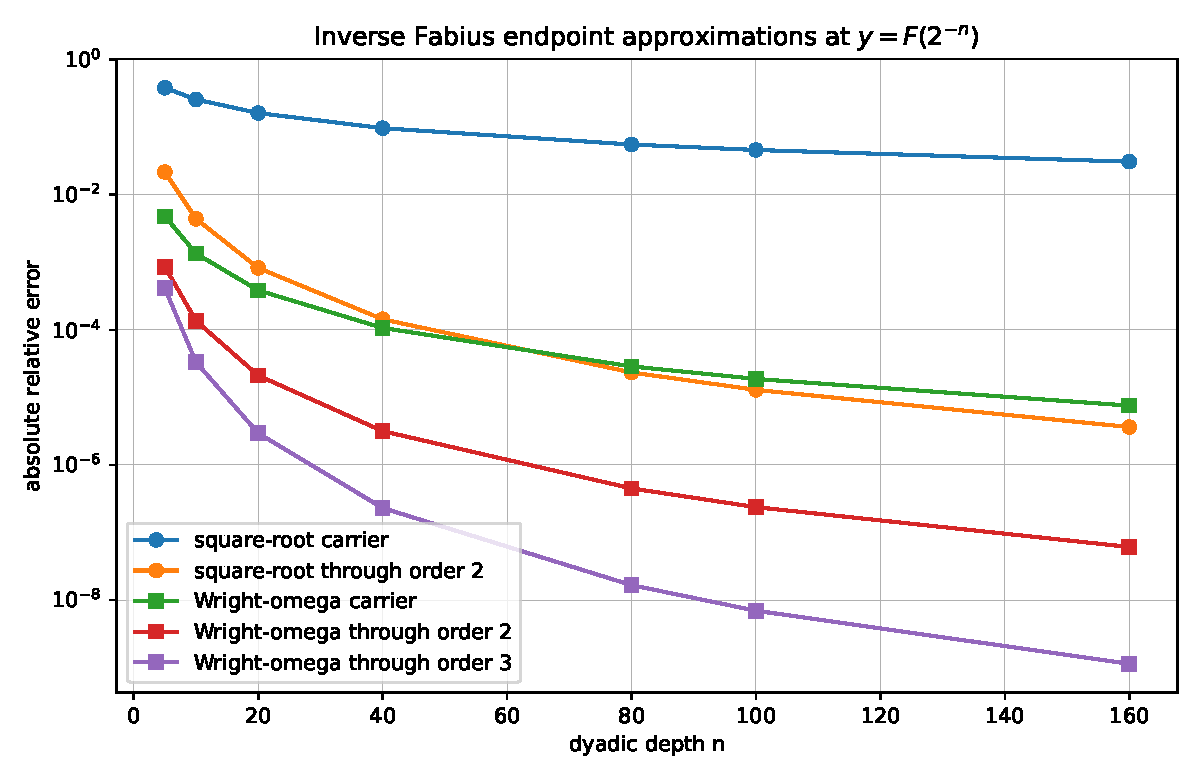
\includegraphics[width=0.78\textwidth]{carrier_comparison.pdf}\\[0.3em]
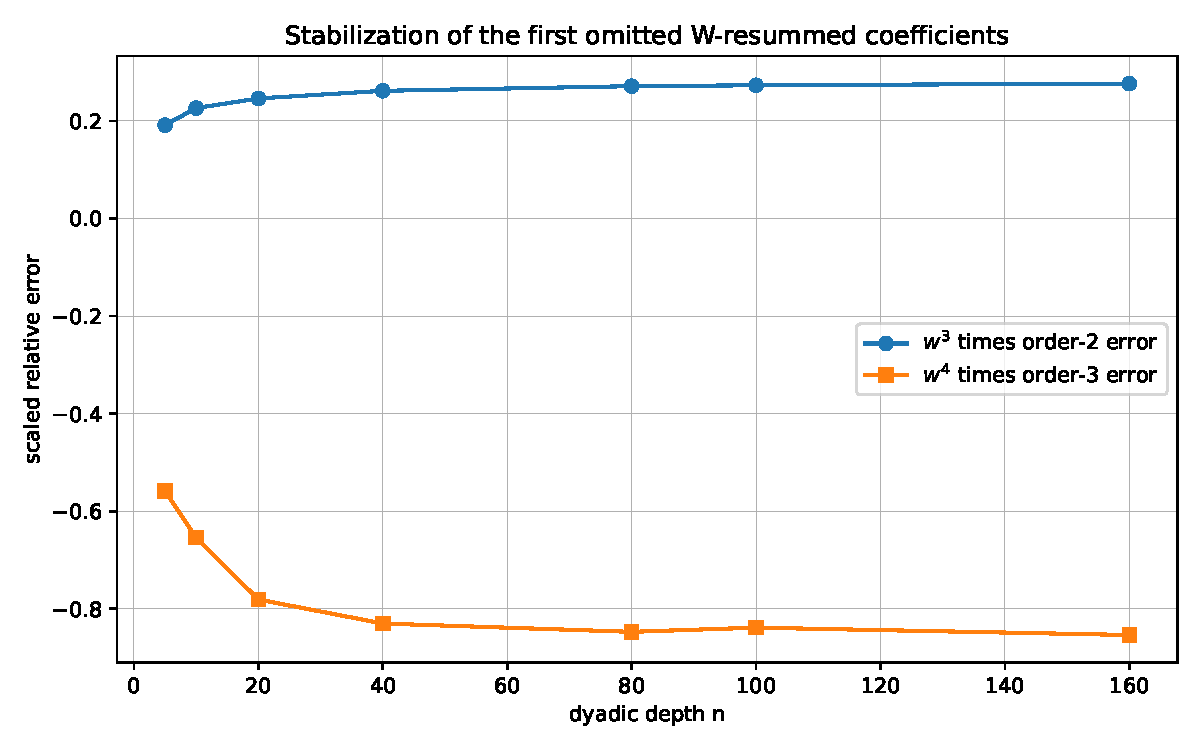
\includegraphics[width=0.78\textwidth]{scaled_residuals.pdf}
\caption{Top: absolute relative errors of the $\rho$- and W-carrier
approximants on the exact dyadic quantiles.  Bottom: scaled residuals
after the second and third W-corrections, consistent with the
predicted next powers $w^{-3}$, $w^{-4}$.}
\label{fig:W-figures}
\end{figure}

\begin{remark}[Pre-asymptotic hierarchy]
Since $\norm{\Psi}_\infty\approx2.13\times10^{-6}$ while
$h_2^{(0)}=5/24$, the nominally first correction $h_1/w=-\Psi/w$ is
numerically \emph{invisible} against $h_2/w^{2}$ until
$w\gtrsim(5/24)/\norm{\Psi}_\infty\approx10^{5}$, i.e.\
$T\sim3\times10^{9}$.  Practical approximations must therefore
include $h_2$ whenever they include $h_1$
(cf.\ the table's near-identical first two columns).  This does not
violate asymptotic ordering; one coefficient simply happens to be
extraordinarily small --- the same smallness that makes the phase
oscillation resolvable only at high precision.
\end{remark}

\begin{remark}[Two beyond-all-orders scales, sharpened]
The W-normalization cleanly separates the two sectors of
\cref{conj:transseries}: a doubly exponential dyadic tail
$\bigO(w^{-1}\e^{-2^{\vartheta}})$ (a forward perturbation of size
$\e^{-2^{\lambda}}$, divided by the steep phase derivative $Lw$) and
the saddle-resurgent scale.  For the latter, optimizing the
amplitude law \eqref{eq:amplitude-law} against the Fourier decay
$\abs{\Psihat(k)}\asymp\e^{-\pi^{2}\abs k/L}$ places the dominant
mode of $g_m$ near $k_*\sim2(m-1)L/\pi^{2}$ and gives the linearized
growth $m!\,(8/\pi^{2})^{m}$ up to algebraic factors --- optimal
truncation near $m\simeq\pi^{2}w/8$ with remainder scale
$\exp(-\pi^{2}w/8)$, enormously larger than the dyadic sector.  This
sharpens \cref{conj:gevrey} to the limsup form
$\limsup_m(\norm{g_m}/m!)^{1/m}=8/\pi^{2}$ (after removing finitely
many low orders and in a suitable norm) and
\cref{conj:optimal-truncation} to Borel one-summability on the
positive $w$-ray with nearest singularities at modulus
$\pi^{2}/8$ (\cref{conj:transseries}); locating the exact branch
point of the bare skeleton \eqref{eq:bare-series} --- an explicit
elimination problem --- would separate the geometric carrier growth
from the factorial saddle growth rigorously.
\end{remark}

\section{The forward saddle engine: constrained partition sums}
\label{sec:saddle}

The inverse formulas consume the periodic forward coefficients
$A_j$.  This chapter closes their construction with a finite
partition formula for the universal Gaussian layer of the saddle
analysis of the Bromwich integral.

Let $s>0$ solve the saddle equation $x=-K'(s)$ and normalize the
saddle jets and their ratios
\begin{equation}
 \varkappa_r=s^{r}K^{(r)}(s),
 \qquad
 \varrho_r=\frac{\varkappa_r}{\varkappa_2}
 \quad(r\ge3).
 \label{eq:saddle-jets}
\end{equation}
Scaling the contour by $t=s(1+\ii Z/\sqrt{\varkappa_2})$,
$Z\sim N(0,1)$, produces the formal correction factor
\begin{equation}
 \mathcal S=\E\left[
 \Bigl(1+\frac{\ii Z}{\sqrt{\varkappa_2}}\Bigr)^{-1}
 \exp\Bigl(\sum_{r\ge3}\frac{\varrho_r}{r!}
 \frac{(\ii Z)^{r}}{\varkappa_2^{(r-2)/2}}\Bigr)
 \right]
 \sim1+\sum_{n\ge1}\frac{C_n}{\varkappa_2^{\,n}},
 \label{eq:S-def}
\end{equation}
the reciprocal factor being the CDF's Bromwich $1/t$ --- deleting it
would produce the \emph{density} coefficients instead.

\begin{theorem}[Constrained-partition formula]
\label{thm:Cn}
For $n\ge1$,
\begin{equation}
 \boxed{\;
 C_n=\sum_{\substack{m_0,m_3,m_4,\dots\ge0\\
 m_0+\sum_{r\ge3}(r-2)m_r=2n}}
 (-1)^{m_0+N/2}\,(N-1)!!\,
 \prod_{r\ge3}\frac{\varrho_r^{\,m_r}}{m_r!\,(r!)^{m_r}},
 \qquad
 N:=m_0+\sum_{r\ge3}rm_r,
 \;}
 \label{eq:Cn-partition}
\end{equation}
a finite sum (the constraint forces $N$ even and $r\le2n+2$).  When
all $\varrho_r$ vanish it reduces to the Gaussian Mills-ratio
coefficients $C_n=(-1)^{n}(2n-1)!!$ --- a sensitive sign and
normalization check, verified symbolically ($-1,3,-15$).  The
logarithmic coefficients
$\log\mathcal S\sim\sum\Lambda_n\varkappa_2^{-n}$ follow
nonrecursively from
\begin{equation}
 \Lambda_n=\sum_{k=1}^{n}\frac{(-1)^{k-1}}k
 \sum_{n_1+\dots+n_k=n,\;n_j\ge1}
 C_{n_1}\cdots C_{n_k},
 \qquad
 \Lambda_1=C_1,\quad
 \Lambda_2=C_2-\tfrac12C_1^{2}.
 \label{eq:Lambda}
\end{equation}
\end{theorem}

\begin{proof}
Expand the reciprocal geometrically ($m_0$ factors of
$-\ii Z/\sqrt{\varkappa_2}$) and the exponential by multiplicities
$m_r$.  The total inverse half-power of $\varkappa_2$ is
$\tfrac12(m_0+\sum(r-2)m_r)$, giving the constraint; the Gaussian
degree is $N$ with $N-2n=2\sum m_r$ even, so
$\E Z^{N}=(N-1)!!$; the powers of $\ii$ and the reciprocal's sign
give $(-1)^{m_0+N/2}$; and the exponential series supplies the
multiplicity factorials.  The $\Lambda$ formula is
$\log(1+\cdot)$ composed with the $C$-series.
\end{proof}

The first coefficients are
$C_1=-1-\tfrac12\varrho_3+\tfrac18\varrho_4
-\tfrac5{24}\varrho_3^{2}$ and
\begin{equation}
 C_2=3+\tfrac52\varrho_3-\tfrac58\varrho_4+\tfrac18\varrho_5
 -\tfrac1{48}\varrho_6
 +\tfrac{35}{24}\varrho_3^{2}-\tfrac{35}{48}\varrho_3\varrho_4
 +\tfrac7{48}\varrho_3\varrho_5+\tfrac{35}{384}\varrho_4^{2}
 +\tfrac{35}{48}\varrho_3^{3}
 -\tfrac{35}{64}\varrho_3^{2}\varrho_4
 +\tfrac{385}{1152}\varrho_3^{4}.
 \label{eq:C2}
\end{equation}
With $q=\log_2s$ and $J(q)=K(2^{q})$, the normalized jets are
generated exactly by the operator identity
$\varkappa_r(q)=L^{-r}\prod_{j=0}^{r-1}(D_q-jL)\,J(q)$; inserting
the exact decomposition of $K$ from
\cref{sec:dyadic-completion} and converting from the saddle
coordinate $q$ to the exact Lambert phase completes the pipeline
\begin{equation}
 \Psi
 \;\longrightarrow\;\{\varkappa_r\}
 \;\xrightarrow{\eqref{eq:Cn-partition}}\;\{C_n\}
 \;\xrightarrow{\eqref{eq:Lambda}}\;\{\Lambda_n\}
 \;\longrightarrow\;\{A_j\}
 \;\xrightarrow{\eqref{eq:diagonal-dn}}\;\{d_n\}
 \;\xrightarrow{\eqref{eq:gn-direct}}\;\{g_n\},
 \label{eq:pipeline}
\end{equation}
every arrow a finite differential-polynomial or
coefficient-extraction operation at fixed order.  The raw term count
of \eqref{eq:Cn-partition} grows like an integer-partition function
--- subexponentially --- rather than like all set partitions, which
removes the practical bottleneck to generating $A_3,A_4,\dots$ in
compact Fourier-differential form.

For implementers, the corpus also supplies a second, fully unrolled
closed route to the same $A_j$ (recorded in the third absorbed
source from the archived small-argument study): with the signed
Stirling coefficients $\prod_{r=1}^{n}(z-r)=\sum_mc(n,m)z^{m}$ and
harmonic numbers $\Hnum_n$, the bounded saddle jets are
\begin{equation}
 q_n(u)=(-1)^{n}n!\Bigl(\frac{\Hnum_n}{L}-\frac12\Bigr)
 +\sum_{m=0}^{n}c(n,m)\,\frac{\Psi^{(m+1)}(u)}{L^{m+1}},
 \label{eq:qn-jets}
\end{equation}
the normalized mass coefficients $a_j$ are finite sums over
compositions of $2j$ and subsets weighted by double factorials
$(2j+2\abs S-1)!!$, and
$A_j=\sum_{r\le j}\frac{(-1)^{r-1}}r
\sum_{\mathcal C(j,r)}a_{s_1}\cdots a_{s_r}$ --- an explicit finite
differential polynomial in $\Psi',\dots,\Psi^{(2j)}$ whose top jet
reproduces \eqref{eq:A1-and-topjet}.  The partition engine
\eqref{eq:Cn-partition} and this composition route validate each
other symbolically.

\section{The exact \texorpdfstring{$2$}{2}-adic completion of the
Laplace exponent}
\label{sec:dyadic-completion}

Everything so far is asymptotic in $\rho$.  This chapter is
\emph{exact}: it completes the quadratic--periodic normal form of
$K$ by an explicitly $2$-adic, everywhere-convergent tail, and shows
that the periodic phase and the beyond-all-orders sectors are two
faces of one Mellin kernel.

\subsection{The decomposition and the dyadic Bose tail}

The product \eqref{eq:K-def} gives the dyadic difference equation
$K(2t)-K(t)=\log(1-\e^{-t})-\log t$.  Define the \emph{dyadic Bose
tail}
\begin{equation}
 B(t)=-\sum_{k\ge0}\log\bigl(1-\e^{-2^{k}t}\bigr),
 \qquad
 B(t)=-\log(1-\e^{-t})+B(2t).
 \label{eq:B-def}
\end{equation}

\begin{theorem}[Exact quadratic--periodic--dyadic decomposition]
\label{thm:K-decomposition}
For every $t>0$,
\begin{equation}
 \boxed{\;
 K(t)=-\frac{\log^{2}t}{2L}+\frac12\log t-\CB
 +\Psi(\log_2t)+B(t).
 \;}
 \label{eq:K-decomposition}
\end{equation}
\end{theorem}

\begin{proof}
With $Q(q)=-\tfrac L2q^{2}+\tfrac L2q$ one checks
$Q(q+1)-Q(q)=-Lq$, so
$\Omega(q):=K(2^{q})-Q(q)-B(2^{q})$ is $1$-periodic by the two
difference equations.  The small-$t$ Mellin expansion of $B$
(\cref{thm:mellin-bridge} below) is
$B(t)=\log^{2}(1/t)/(2L)+\tfrac12\log(1/t)+\CB-\Psi(\log_2t)+
\smallo(1)$, and $K(t)\to0$ as $t\downarrow0$; letting
$q=m+u\to-\infty$ at fixed $u$ identifies
$\Omega(u)=\Psi(u)-\CB$, and periodicity upgrades the identity to
all $q$.
\end{proof}

\begin{theorem}[Exact $2$-adic coefficients]
\label{thm:B-2adic}
For every $t>0$,
\begin{equation}
 \boxed{\;
 B(t)=\sum_{n\ge1}b_n\,\e^{-nt},
 \qquad
 b_n=\frac{2^{\vtwo(n)+1}-1}{n},
 \;}
 \qquad
 0<b_n<2,
 \label{eq:B-2adic}
\end{equation}
with the elementary tail enclosure
$0<B(t)-\sum_{n\le N}b_n\e^{-nt}\le2\e^{-(N+1)t}/(1-\e^{-t})$.
\end{theorem}

\begin{proof}
Expand each Bose logarithm and regroup
$B(t)=\sum_{k\ge0}\sum_{m\ge1}m^{-1}\e^{-m2^{k}t}$: the
representations $n=m2^{k}$ are indexed by $0\le k\le\vtwo(n)$, with
total weight
$\tfrac1n\sum_{k\le\vtwo(n)}2^{k}=(2^{\vtwo(n)+1}-1)/n$.
\end{proof}

The first terms,
$B(t)=\e^{-t}+\tfrac32\e^{-2t}+\tfrac13\e^{-3t}
+\tfrac74\e^{-4t}+\tfrac15\e^{-5t}+\tfrac12\e^{-6t}+\cdots$, spike at
powers of two: the exact arithmetic trace of the dyadic scale
hierarchy.  The integer weight $f(n)=nb_n=2^{\vtwo(n)+1}-1$
satisfies $f(2n)=2f(n)+1$, $f(2n+1)=1$, and its generating function
obeys the Mahler equation $C(z)=2C(z^{2})+z/(1-z)$, placing the
sectors in the same digital universe as the Thue--Morse and ruler
sequences --- but with geometric accumulation over the full
$2$-adic valuation in place of digit-sum parity.  Note the
crosswalk: $\vtwo(n)+1$ is precisely the integer zero order of
$\widehat\Up$ that drives the exactness theorems of the companion
volume \emph{Dyadic-Comb Frontiers}; here the same statistic returns
as the arithmetic seed of the beyond-all-orders sectors.

\subsection{One Mellin kernel, two asymptotic ends}

\begin{theorem}[Mellin bridge]
\label{thm:mellin-bridge}
For $\Re s>0$,
\begin{equation}
 \sum_{n\ge1}\frac{b_n}{n^{s}}
 =\frac{\zeta(s+1)}{1-2^{-s}},
 \qquad
 \int_0^\infty B(t)\,t^{s-1}\dd t
 =\Gamma(s)\,\frac{\zeta(s+1)}{1-2^{-s}},
 \label{eq:mellin}
\end{equation}
and contour shifting in the Mellin inversion gives, for every fixed
$M$, with $R=\log(1/t)$,
\begin{equation}
 B(t)=\frac{R^{2}}{2L}+\frac R2+\CB-\Psi(\log_2t)
 +\sum_{m=1}^{M-1}\frac{(-1)^{m}\zeta(1-m)}{m!\,(1-2^{m})}\,t^{m}
 +\bigO_M(t^{M})
 \qquad(t\downarrow0).
 \label{eq:B-small-t}
\end{equation}
\end{theorem}

\begin{proof}
The Dirichlet series is the double sum
$\sum_{k}\sum_{m}m^{-1}(m2^{k})^{-s}
=\zeta(s+1)\sum_k2^{-ks}$; termwise Mellin transformation of
\eqref{eq:B-2adic} gives the transform.  Shifting the inversion
contour left: the order-three pole at $s=0$ of
$\Gamma(s)\zeta(1+s)(1-2^{-s})^{-1}$ yields the quadratic polynomial
and $\CB$; the simple poles at $s=\chi_k$ yield exactly
$-\Psi(\log_2t)$ by \eqref{eq:Psi-Fourier}; and the poles of
$\Gamma$ at $-m$ yield the Bernoulli-type powers.
\end{proof}

\begin{statusbox}{Two faces of one kernel}
The Gamma--zeta phase $\Psi$ (small-$t$ residues at the complex
dimensions $2\pi\ii k/L$) and the exact $2$-adic exponential sectors
(large-$t$ Dirichlet regrouping) are generated by the \emph{same}
kernel $\Gamma(s)\zeta(s+1)/(1-2^{-s})$.  No new frequencies ever
appear downstream: the entire hierarchy of inverse oscillations
consists of integer convolutions of the modes
$\chi_k$ (\cref{prop:convolutions}), and the beyond-all-orders
remainder is not an opaque error but the explicit arithmetic object
\eqref{eq:B-2adic}.  As a byproduct, comparing the two derivations
of the constant term proves $\Csharp+\CB=-\tfrac12\log(2\pi)$.
\end{statusbox}

\subsection{Exact saddle map and ultraflat jets}

\begin{corollary}[Exact $2$-adic saddle map]
\label{cor:saddle-map}
With $t=2^{q}$, the saddle abscissa $x=-K'(t)$ is exactly
\begin{equation}
 \boxed{\;
 x(q)=2^{-q}\Bigl(q-\frac12-\frac{\Psi'(q)}{L}\Bigr)
 +\sum_{n\ge1}\bigl(2^{\vtwo(n)+1}-1\bigr)\,\e^{-n2^{q}},
 \;}
 \label{eq:saddle-map}
\end{equation}
the first term the complete algebraic--periodic saddle map, the
second an exact convergent ultraflat correction.  Derivative
bookkeeping is closed: with Stirling numbers of the second kind,
\begin{equation}
 \frac{\dd^{r}}{\dd q^{r}}B(2^{q})
 =L^{r}\sum_{n\ge1}b_n
 \sum_{j=0}^{r}
 \genfrac\{\}{0pt}{}{r}{j}\,(-n2^{q})^{j}\,\e^{-n2^{q}},
 \qquad
 t^{r}B^{(r)}(t)=(-1)^{r}\sum_{n\ge1}b_n\,(nt)^{r}\e^{-nt}.
 \label{eq:touchard-jets}
\end{equation}
\end{corollary}

The jet formulas expose the technical obstacle to naive
hyperasymptotics: each $q$-derivative of an
$\e^{-n2^{q}}$ sector produces powers of $2^{q}$, so the ordinary
inverse-power saddle hierarchy is \emph{not uniform} inside a fixed
dyadic sector; and although the algebraic inversion gives the saddle
coordinate $q_\star(y)=\theta+\bigO(\ell/\rho)$, the induced change
in the exponent $n2^{q_\star}$ is of order
$2^{\theta}\ell/\rho\to\infty$ --- the exact saddle coordinate is
part of the beyond-all-orders datum
(\cref{conj:transseries}).

\section{Verification}
\label{sec:verification-inv}

The two absorbed packages verify overlapping claims by independent
implementations; both suites live under \nolinkurl{assets/}.

\emph{Symbolic.}  Over algebraically independent symbols
$L,\beta,\Csharp,\ell,P_0,\dots,P_4,A_1,A_1',A_2$, both codes confirm
$d^{\mathrm{diagonal}}_j-d^{\mathrm{triangular}}_j\equiv0$
($j\le3$), the third correction \eqref{eq:d3}, the universal top-log
\eqref{eq:universal-top-log}, and the top-jet transfer
\eqref{eq:inverse-topjet}; the saddle generator reproduces
$C_n=(-1)^{n}(2n-1)!!$ at vanishing $\varrho$ and archives
$C_1,C_2,C_3,\Lambda_2$ (\nolinkurl{generated_coefficients.tex}).

\emph{Exact identities.}  At $70$--$100$ digits, the decomposition
\eqref{eq:K-decomposition} agrees with the defining product for
$K$ to $\sim10^{-16}$ at $t\in\{0.1,1,3,10\}$ (twelve Fourier
modes); the $2$-adic series \eqref{eq:B-2adic} agrees with the
product to $7.5\times10^{-39}$ at $t=0.7$ and
$3.8\times10^{-55}$ at $t=1.5$; the small-$t$ expansion
\eqref{eq:B-small-t} to $\sim4\times10^{-16}$ on
$0.02\le t\le0.2$; and the Dirichlet identity
\eqref{eq:mellin} to the expected algebraic truncation tail with
$5\times10^{4}$ unaccelerated terms.

\emph{Wright-omega layer.}  The third source's suite independently
reconstructs the W-scale $d_m,h_m,g_m$ symbolically from the residual
equation (SymPy; the identities of
\cref{sec:wcarrier} including the $5/24$ cancellation and the
zero-periodic values \eqref{eq:zero-periodic}), verifies the carrier
equation and Newton evaluation of $\omega$, and generates the
carrier-comparison tables of \cref{tab:W-errors} on the same exact
dyadic quantiles at $100$ digits with nine Fourier modes.

\emph{Exact dyadic quantiles.}  With $a_0=1$ and
$a_n=(2^{n}-1)^{-1}\sum_{k<n}a_k/(n-k+1)!$, the repository's exact
values give $y_n=F(2^{-n})=2^{-n(n-1)/2}a_n$ with
$G(y_n)=2^{-n}$ \emph{exactly} --- no inversion error, only the
asymptotic formula is evaluated (at $100$ digits, twelve modes).
Signed relative errors of $G^{[r]}
=\Gzero\exp(\sum_{j\le r}h_j\rho^{-j})$:

\begin{center}
\small
\begin{tabular}{@{}rrrrrr@{}}
\toprule
$n$ & $\rho$ & $\Gzero$ only & through $h_1$ & through $h_2$ & through $h_3$ \\
\midrule
5   & 6.44   & $-3.83\times10^{-1}$ & $7.89\times10^{-2}$ & $-2.17\times10^{-2}$ & $6.41\times10^{-3}$ \\
10  & 12.08  & $-2.57\times10^{-1}$ & $2.69\times10^{-2}$ & $-4.40\times10^{-3}$ & $7.19\times10^{-4}$ \\
20  & 22.82  & $-1.62\times10^{-1}$ & $8.76\times10^{-3}$ & $-8.24\times10^{-4}$ & $7.40\times10^{-5}$ \\
40  & 43.65  & $-9.66\times10^{-2}$ & $2.72\times10^{-3}$ & $-1.43\times10^{-4}$ & $6.96\times10^{-6}$ \\
80  & 84.54  & $-5.53\times10^{-2}$ & $8.05\times10^{-4}$ & $-2.34\times10^{-5}$ & $6.05\times10^{-7}$ \\
120 & 125.08 & $-3.94\times10^{-2}$ & $3.88\times10^{-4}$ & $-7.92\times10^{-6}$ & $1.40\times10^{-7}$ \\
160 & 165.47 & $-3.08\times10^{-2}$ & $2.30\times10^{-4}$ & $-3.64\times10^{-6}$ & $4.92\times10^{-8}$ \\
\bottomrule
\end{tabular}
\captionof{table}{Exact-quantile tests: the new third correction
improves the two-correction error by factors $11$--$74$ across the
tested range.}
\label{tab:dyadic-errors}
\end{center}

\begin{figure}[htbp]
\centering
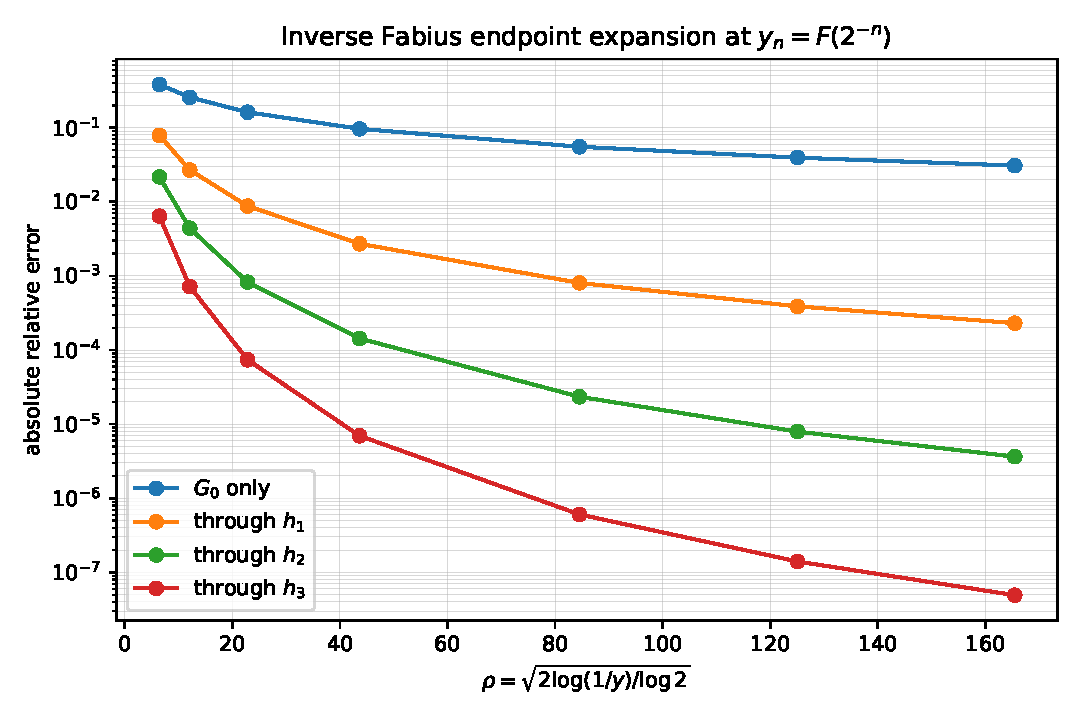
\includegraphics[width=0.78\textwidth]{endpoint_error_plot.pdf}
\caption{Absolute relative errors on the exact dyadic quantiles;
each added logarithmic correction produces the expected strong
reduction once $\rho$ is moderately large.}
\label{fig:error-plot}
\end{figure}

\begin{figure}[htbp]
\centering
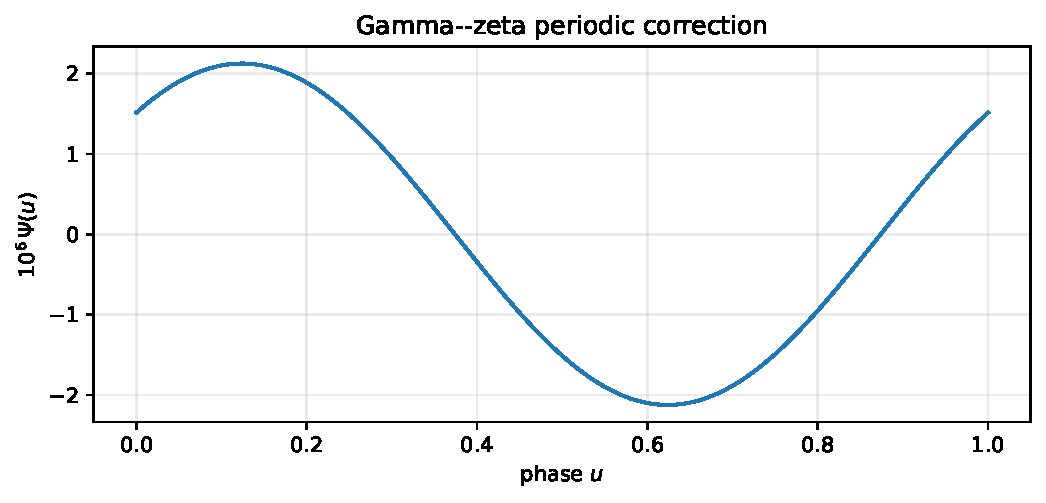
\includegraphics[width=0.72\textwidth]{psi_periodic.pdf}\\[0.35em]
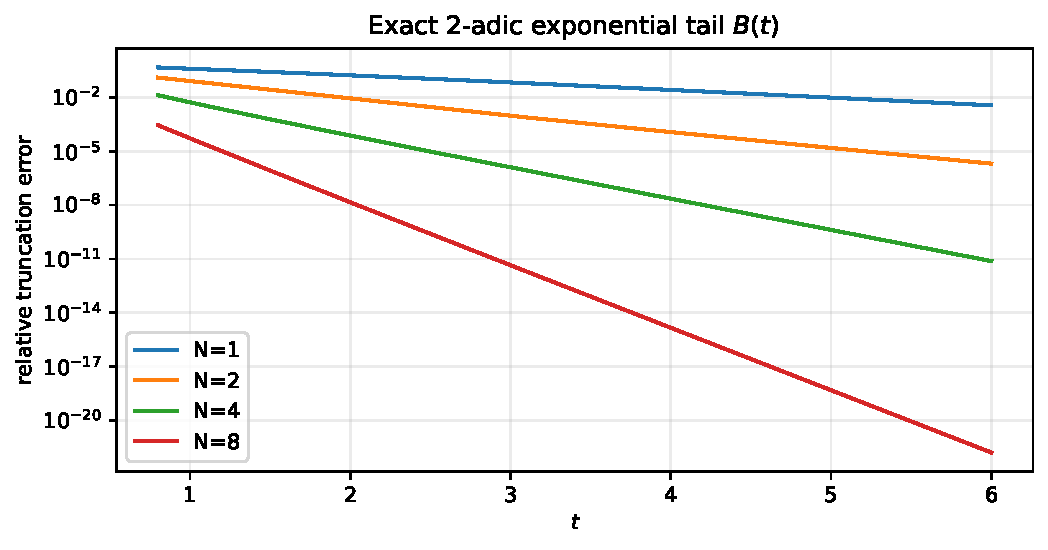
\includegraphics[width=0.72\textwidth]{dyadic_tail_convergence.pdf}
\caption{Top: the centered Gamma--zeta fluctuation $\Psi$ --- tiny
amplitude, same asymptotic order as the constants.  Bottom: relative
error of $N=1,2,4,8$ terms of the exact $2$-adic series for
$B(t)$, with the elementary enclosure of
\cref{thm:B-2adic}.}
\label{fig:psi-and-tail}
\end{figure}

\section{Connections across the corpus}
\label{sec:connections-inv}

\emph{Literal small-$y$ form.}  Substituting
$\rho=\sqrt{2T/L}$ back, the complete expansion reads
\begin{equation}
 G(y)=\frac{\sqrt T}{\e\sqrt L}\,\e^{-\sqrt{2LT}}
 \exp\Bigl\{\sum_{n=1}^{N}
 \Bigl(\frac{L}{2T}\Bigr)^{n/2}
 h_n\bigl(\tfrac12\log\tfrac{2T}L,\;
 \sqrt{2T/L}+\beta\bigr)\Bigr\}
 \Bigl[1+\bigO_N\Bigl(\frac{(1+\log T)^{N}}{T^{(N+1)/2}}\Bigr)\Bigr].
 \label{eq:literal}
\end{equation}
\emph{Lambert geometry.}  The method performs the saddle inversion in
$\lambda$ and invokes the exact Lambert identity only once, through
\eqref{eq:ratio-exact}: that is why the coefficients are polynomial
in the single logarithm $\ell$ rather than an uncontrolled nest, and
why $\beta$ (which completes the square in the dominant exponent) is
the only constant shift.  \emph{Bell structures.}  Two Bell
mechanisms compose without flattening: the forward
$A_j$ are Bell assemblies of saddle jets, the inverse $g_n$ are Bell
assemblies of the $h_j$ --- the diagonal formula is the
``Bell-of-Bell'' transform with a diagonal grading.
\emph{Thue--Morse and $q$-data.}  The exact dyadic quantiles that
verify the expansion are the same $q$-binomial arithmetic that runs
the companion volumes; the $2$-adic seed
$b_n$ shares its statistic $\vtwo(n)+1$ with the sinc zero orders;
and the up-function reading of the expansion is geometric: it is the
all-orders law of the inward displacement from the support boundary
of the Rvachev bell at prescribed tiny height, the Gamma--zeta
oscillation being the Mellin shadow of the same dyadic lattice that
generates the sinc product.

\section{Conjectures and frontier directions}
\label{sec:conjectures-inv}

\begin{conjecture}[Gevrey-one growth]
\label{conj:gevrey}
On compact real phase sets (and in weighted analytic norms on a
strip, with weight $1+\abs\ell$ for the polynomial part),
$\abs{h_n}+\abs{g_n}\le CA^{n}n!$.  The top-jet transfer
\eqref{eq:inverse-topjet} combined with a Cauchy estimate at the
strip boundary $\pi/(2L)$ gives the heuristic exponential constant
$8/\pi^{2}$ --- a Gevrey-one, not worse, divergence --- but other
saddle diagrams may reinforce or partially cancel it.
\end{conjecture}

\begin{conjecture}[Optimal truncation]
\label{conj:optimal-truncation}
At fixed real phase, truncation near
$N_{\mathrm{opt}}\sim(\pi^{2}/8)\rho$ leaves an exponentially small
remainder whose leading exponential and Stokes data are governed by
the nearest complex singularities of $\Psi$ and the lower-Lambert
branch geometry.
\end{conjecture}

\begin{conjecture}[Sharp strip inheritance]
\label{conj:strip-sharp}
Each periodic coefficient of $d_n,h_n,g_n$ extends to the same
maximal strip as $\Psi$ and no generic cancellation enlarges it: the
Fourier decay rate is stable under all inverse operations.
\end{conjecture}

\begin{conjecture}[Nonconstant phase at every order]
\label{conj:nonconstant-phase}
Every $d_n,h_n,g_n$ has a nonconstant periodic component for generic
$\ell$: no finite truncation beyond the elementary factor is
phase-blind.  (The top-jet law makes this overwhelmingly plausible;
a certified proof could isolate the $\abs k=1$ modes against the
enormous decay gap to $\abs k\ge2$.)  At higher orders the
renormalized phase profiles trace closed analytic curves; for generic
jet selections these should be immersed, and for rich selections
embedded, with embedding dimension controlled by the first
Gamma--zeta modes --- a ``quantile cluster geometry.''
\end{conjecture}

\begin{conjecture}[Two-level exponentially improved transseries]
\label{conj:transseries}
After optimal truncation, $G(y)$ admits an exponentially improved
description with at least two distinct levels: saddle-resurgent
sectors controlled by the large-order growth of the $A_j$, and
ultraflat dyadic sectors
$\exp(-n2^{\,q_\star(y)})$ seeded by
$b_n=(2^{\vtwo(n)+1}-1)/n$, where $q_\star$ is the \emph{exact}
saddle coordinate of \eqref{eq:saddle-map} (not replaceable by
$\theta$; see \cref{sec:dyadic-completion}).  Within the ultraflat
level, the Stokes/connection data should be Dirichlet convolutions
of $b_n$, i.e.\ finite products of
$\zeta(s+1)/(1-2^{-s})$ and shifts --- a precise, computationally
testable resurgent-arithmetic prediction.
\end{conjecture}

\begin{conjecture}[Universal diagonal inversion class]
\label{conj:universal-class}
Whenever a distribution has a forward exact-phase expansion
$-a\lambda^{2}+b\lambda-c\log\lambda+C+P(\lambda)
+\sum A_j(\lambda)\lambda^{-j}$ with periodic analytic
$P,A_j$, its inverse admits the entire package proved here ---
diagonal expansion with polynomial logarithms, phase locking,
newest-jet transfer, Bell conversion --- with universal highest
logarithms depending only on $a$ and $c$.  For base
$b>1$ smoothing laws the $2$-adic tail generalizes with coefficients
$(b^{\nu_b(n)+1}-1)/((b-1)n)$ and kernel
$\zeta(s+1)/(1-b^{-s})$, the phase acquiring period one in
$\log_b$.
\end{conjecture}

Concrete projects: generate $A_3,A_4$ compactly through the pipeline
\eqref{eq:pipeline} and make $g_4,g_5$ explicit in $\Psi$ alone;
prove weighted Wiener-algebra bounds uniform in phase; run optimal
truncation experiments to see whether the first visible
beyond-all-orders scale is saddle-resurgent or the far smaller
dyadic one; quantify the uniform-in-$m$ breakdown of the derivative
law \eqref{eq:two-term-derivative}; locate the nearest complex
critical values of $F$ (the analytic continuation radius of $G$ and
the Borel singularities); and build certified few-mode
Fourier-polynomial coefficient tables
$g_n\approx\sum_{r\le n}\sum_{\abs k\le K}c_{n,r,k}\ell^{r}
\e^{2\pi\ii k\theta}$ that, with one Newton step on the exact
functional equation, give a fast globally certified quantile
algorithm.

\begin{statusbox}{Lean formalization roadmap}
Four layers, the first three purely formal:
(1) a two-scale coefficient ring (truncated series over
$\R[\ell]\otimes C^\infty(\R/\Z)$, closure under composition, log,
exp); (2) parameterized Lagrange inversion
$[t^{k}]W=\tfrac1k[w^{k-1}]\Phi^{k}$ and the diagonal specialization
\eqref{eq:diagonal-dn}; (3) the Gaussian contraction
\eqref{eq:Cn-partition} over an algebraic moment functional, and the
$2$-adic regrouping and Dirichlet identities of
\cref{sec:dyadic-completion} (a bijection and two Tonelli
arguments); (4) the analytic transfer
(\cref{app:proof-details}) from formal cancellation to the
fixed-order remainder.  The degree/top-jet filtrations of
\cref{sec:structure} are finite combinatorics on top of (2).
\end{statusbox}

\appendix

\section{Proof details}
\label{app:proof-details}

\emph{Finiteness bookkeeping.}  In \eqref{eq:diagonal-dn} the index-$k$
summand requests $z^{\,n-k}w^{\,k-1}$: no $\Phi$-power beyond
$z^{\,n-k}$, no Taylor jet beyond order $k-1$, and $A_j$ only for
$j\le n-k$; hence $A_{n-1}$ occurs only at $k=1$ --- the key to the
top-jet proof.

\emph{Formal-to-asymptotic transfer.}  With
$\mathscr F(w)=\tfrac Lzw+\mathcal R_N(w)+E_N(w)$,
$E_N=\bigO_N(z^{N})$, formal cancellation gives
$\mathscr F(D^{[N]})=\bigO_N((1+\ell)^{N}z^{N})$, while
$\inf\abs{\partial_w\mathscr F}\ge L/(2z)$ throughout the relevant
$\bigO(\ell z)$ neighborhood for small $z$; hence
$\abs{D-D^{[N]}}\le(2z/L)\abs{\mathscr F(D^{[N]})}
=\bigO_N((1+\ell)^{N}z^{N+1})$ --- the gain-of-one-power argument
that lets a forward expansion through $A_{N-1}$ certify an inverse
expansion through $d_N$.  The map
$\lambda\mapsto\lambda\e^{-L\lambda}$ then transfers phase error to
relative inverse error of the same order.

\section{Coefficient dictionary}
\label{app:dictionary}

\begin{align*}
 L&=\log2,
 &\beta&=\tfrac1L+\tfrac12,
 &T&=\log(1/y),
 &\rho&=\sqrt{2T/L},\\
 z&=\rho^{-1},
 &\ell&=\log\rho,
 &\theta&=\rho+\beta,
 &\Gzero&=\rho\,\e^{-L\rho-L\beta},\\
 \lambda&=\rho+\beta+D,
 &D&=\textstyle\sum d_nz^{n},
 &d_n&=\textstyle\sum_{k=1}^{n}\frac{(-1)^{k}}{kL^{k}}
 [z^{n-k}w^{k-1}]\mathcal R^{k},
 &\tfrac G{\Gzero}&=(1+\beta z+zD)\e^{-LD},
\end{align*}
with $\mathcal R$ from \eqref{eq:R-def}; these lines suffice to
implement the complete inverse expansion once the forward
$A_j$ are available (\cref{sec:saddle}).  In evaluation: preserve the
exact phase $\theta=\rho+\beta$ inside every periodic coefficient
(replacing it by $\rho$ shifts the first oscillatory correction);
work through $\log G$ at extreme $y$; and use the Fourier form of
$\Psi$, whose differentiated modes keep exponential decay.  For
reference,
\begin{equation}
 \Lambda_2=\tfrac5{16}\varrho_3^{4}+\tfrac58\varrho_3^{3}
 -\tfrac{25}{48}\varrho_3^{2}\varrho_4+\tfrac98\varrho_3^{2}
 -\tfrac23\varrho_3\varrho_4+\tfrac7{48}\varrho_3\varrho_5
 +2\varrho_3+\tfrac1{12}\varrho_4^{2}-\tfrac12\varrho_4
 +\tfrac18\varrho_5-\tfrac1{48}\varrho_6+\tfrac52.
 \label{eq:Lambda2-expanded}
\end{equation}

\section{Provenance of the absorbed sources}
\label{sec:provenance-inv}

\begin{center}
\small
\begin{tabular}{@{}p{0.44\textwidth}p{0.50\textwidth}@{}}
\toprule
Source (directory; SHA-256 of main \texttt{.tex}) & Contribution \\
\midrule
\emph{Closed All-Orders Endpoint Asymptotics for the Inverse Fabius
Function}
(\nolinkurl{inverse_fabius_all_orders_package}; SHA in
\nolinkurl{assets/SHA256SUMS-absorbed.txt})
& Diagonal formulas including the general composition and the
$h_n/g_n$ diagonal forms; fixed-order theorem with logarithmic
remainder grading; degree and top-log laws; inverse top-jet law;
$A_2$, $A_1'$; Fourier convolution algebra, analyticity strip,
certified truncation; phase locking, cluster set, tomography;
elasticity and the $Q_m$ hierarchy with the harmonic-number law;
exact-dyadic-quantile verification (\cref{tab:dyadic-errors},
\cref{fig:error-plot}); Gevrey/optimal-truncation/phase-geometry
conjectures; proof-detail appendices. \\
\addlinespace
\emph{Complete Small-Argument Asymptotics of the Inverse Fabius
Function}
(\nolinkurl{inverse_fabius_asymptotics_report}; SHA in
\nolinkurl{assets/SHA256SUMS-absorbed.txt})
& The closed $d_n$ extractor (independent derivation) and the direct
partial-Bell $g_n$ formula; universal top-log (independent proof);
third correction (independent, verified identical); the
constrained-partition saddle engine, Mills specialization,
$\Lambda_n$ composition, jet operator, pipeline; the exact
$2$-adic completion: $K$-decomposition, dyadic Bose tail, Mahler and
Dirichlet forms, Mellin bridge, $\Csharp+\CB$ relation, exact saddle
map, ultraflat jets; Stirling--Bell ordinary-derivative route;
strip-inheritance/transseries/resurgent-arithmetic conjectures;
formalization obligations; $K$/$B$/Dirichlet verification and the
$\Psi$ and tail-convergence figures. \\
\addlinespace
\emph{Complete Small-Argument Asymptotics of the Inverse Fabius
Function} --- Wright-omega carrier (sixth wave;
\nolinkurl{inverse_fabius_asymptotics_package}; SHA in
\nolinkurl{assets/SHA256SUMS-absorbed.txt})
& The log-free resummation of \cref{sec:wcarrier}: carrier equation
and stable $\omega$ evaluation; bounded-periodic no-log coefficient
theorem with the clean $w^{-N-1}$ remainder; $g_1=-\Psi$, the
universal $5/24$ in $h_2$, and the zero-periodic regression values
through $g_4^{(0)}$; carrier-invariant highest-derivative law and
amplitude law; convergent bare-skeleton theorem; conditional
Gevrey-one transfer; W-scale elasticity; the sharpened
two-sector beyond-all-orders picture and the limsup-$8/\pi^{2}$ and
Borel-summability refinements; carrier-comparison experiments and
figures; the imported closed forward-coefficient route
($q_n$ jets, composition/subset mass coefficients). \\
\bottomrule
\end{tabular}
\end{center}

\emph{What was deduplicated}: the imported forward/inverse corpus
inputs; the two-scale setup; the fixed-point reduction; the closed
$d_n$ formula (proved in the first two sources and re-derived by the
third in its own normalization --- one statement here, applied to
both residuals); the universal top-log (two proofs, both retained in
\cref{thm:top-log}); the third correction (independently derived,
verified algebraically identical --- the merge's cross-validation);
the Bell conversion; the elasticity recurrence (identical in the
first two sources, and structurally re-verified by the third:
its W-scale $d_2$ is the shared recursion specialized to the new
carrier, and its highest-derivative constants coincide with
\eqref{eq:inverse-topjet}, confirming carrier invariance); and the
audit/status scaffolding.  Nothing mathematical was discarded; where
the sources' groupings differ, the compacter form is displayed and
the other recorded in the adjacent remark.  Exact SHA-256 hashes are
in \nolinkurl{assets/SHA256SUMS-absorbed.txt}.

\begin{thebibliography}{99}

\bibitem{Fabius1966}
J.~Fabius,
\newblock A probabilistic example of a nowhere analytic
$C^\infty$-function,
\newblock \emph{Z.\ Wahrscheinlichkeitstheorie Verw.\ Geb.}
\textbf{5} (1966), 173--174.

\bibitem{Rvachev1990}
V.~A.~Rvachev,
\newblock Compactly supported solutions of functional-differential
equations and their applications,
\newblock \emph{Russian Math.\ Surveys} \textbf{45} (1990), no.~1,
87--120.

\bibitem{Corless1996}
R.~M.~Corless, G.~H.~Gonnet, D.~E.~G.~Hare, D.~J.~Jeffrey, and
D.~E.~Knuth,
\newblock On the Lambert $W$ function,
\newblock \emph{Adv.\ Comput.\ Math.} \textbf{5} (1996), 329--359.

\bibitem{Comtet1974}
L.~Comtet,
\newblock \emph{Advanced Combinatorics},
\newblock Reidel, 1974.

\bibitem{GouldenJackson1983}
I.~P.~Goulden and D.~M.~Jackson,
\newblock \emph{Combinatorial Enumeration},
\newblock Wiley, 1983.

\bibitem{FlajoletSedgewick2009}
P.~Flajolet and R.~Sedgewick,
\newblock \emph{Analytic Combinatorics},
\newblock Cambridge University Press, 2009.

\bibitem{deBruijn1981}
N.~G.~de~Bruijn,
\newblock \emph{Asymptotic Methods in Analysis},
\newblock Dover, 1981.

\bibitem{Olver1997}
F.~W.~J.~Olver,
\newblock \emph{Asymptotics and Special Functions},
\newblock A K Peters, 1997.

\bibitem{Wong2001}
R.~Wong,
\newblock \emph{Asymptotic Approximations of Integrals},
\newblock SIAM, 2001.

\bibitem{ParisKaminski2001}
R.~B.~Paris and D.~Kaminski,
\newblock \emph{Asymptotics and Mellin--Barnes Integrals},
\newblock Cambridge University Press, 2001.

\bibitem{Titchmarsh1986}
E.~C.~Titchmarsh,
\newblock \emph{The Theory of the Riemann Zeta-Function}, 2nd ed.,
\newblock Oxford University Press, 1986.

\bibitem{AlloucheShallit2003}
J.-P.~Allouche and J.~Shallit,
\newblock \emph{Automatic Sequences},
\newblock Cambridge University Press, 2003.

\bibitem{ProveItPrimary}
V.~Reshetnikov,
\newblock \emph{The Fabius Function and Rvachev's Up-Function},
\newblock primary exposition in the \texttt{ProveIt} repository,
\repo, snapshot 28 August 2026.

\bibitem{ProveItFrontier}
V.~Reshetnikov,
\newblock \emph{Non-Formalized Research Frontiers for the Fabius
Function},
\newblock \texttt{ProveIt} repository, 2026.

\bibitem{ProveItInverse}
V.~Reshetnikov,
\newblock \emph{Inverse and Sampling Frontiers for the
Fabius--Rvachev System},
\newblock consolidated frontier volume,
\nolinkurl{drafts/inverse-and-sampling/Inverse_and_Sampling_Frontiers/},
2026.

\bibitem{ProveItDyadicComb}
V.~Reshetnikov,
\newblock \emph{Dyadic-Comb Frontiers for the Fabius--Rvachev
System},
\newblock consolidated frontier volume,
\nolinkurl{drafts/inverse-and-sampling/Dyadic_Comb_Frontiers/},
28 August 2026.

\end{thebibliography}

\end{document}
